The field of 21-cm cosmology offers a window to the infant Universe after the formation of the Cosmic Microwave Background~(CMB) and prior to the current epoch of the galaxies. We currently know very little about this period, which is divided into the Dark Ages before the first stars formed, the Cosmic Dawn when the first stars and galaxies formed and the Epoch of Reionization when the abundant neutral hydrogen in the Universe was ionized by stellar UV emission.

Although a potentially lucrative probe of the first galaxies, the 21-cm signal from neutral hydrogen in the early universe remains undetected due to complex experimental and data analysis challenges. This body of work focuses primarily on the latter and comprises two main parts.

The first part details the development of three different algorithms and techniques to improve the prospects of detecting the sky-averaged 21-cm signal from neutral hydrogen 100 - 700 million years after the Big Bang and improve our understanding of the first galaxies.

The 21-cm signal is often described as being `fogged' or overwhelmed by Galactic and extragalactic foregrounds, which are five orders of magnitude bigger than the signal itself. Separation of these two components of the data is crucial, and a method for modelling the foreground is described in \cref{ch:maxsmooth} adapted from \cite{Bevins_maxsmooth_2021}. The detailed algorithm uses quadratic programming to fit functions with constrained derivatives. The algorithm is guaranteed to converge on the optimum solution and is shown to improve on traditionally used methods by a factor of two in runtime. We illustrate the application of the foreground modelling tool to data from the Experiment to Detect the Global EoR Signature~(EDGES) \cite{Bowman_edges_2018} and the Large aperture Experiment to detect the Dark Ages~(LEDA) \cite{Price_LEDA_2018}. The work added to the discussion surrounding the nature of the absorption feature reported as a tentative detection of the 21-cm signal in 2018 by EDGES \cite{Bowman_edges_2018}. Further, it illustrated that sinusoidal systematic structures are a prominent feature in 21-cm data sets and that these need to be appropriately accounted for where present. It also demonstrated the application of the foreground modelling technique as a tool for the detection of previously unaccounted for systematics in data sets, as discussed in \cite{de_lera_acedo_reach_2022}.

The signal itself relies on a complex set of astrophysical processes that are typically modelled using semi-numerical simulations \citep[e.g.][]{Visbal_2012, Fialkov_rich_2014, Cohen_global_2017, Reis_sta_2021}. While useful for gaining an understanding of how the Universe evolved during this period, these simulations can take of the order of a few hours per call, which is impractical for most kinds of data analysis. As a result, the application of neural networks, trained on the semi-numerical simulations, was proposed to speed up signal generation in computationally intensive fitting algorithms. First demonstrated in \cite{Cohen2020}, \cref{ch:globalemu} illustrates an alternative approach to the problem of emulation and is based on \cite{Bevins_globalemu_2021}. The work lead to a factor of 102 improvement in emulation time and approximately a factor of two improvement in accuracy.

As more and more data becomes available, the ability to efficiently combine the constraining power of different data sets, a process which can lead to significant improvements in our understanding of the infant Universe, is becoming crucial. In \cref{ch:margarine}, we detail a framework for performing marginal Bayesian inference and calculating marginal Bayesian statistics using Normalising Flows and Kernel Density Estimators. The chapter is adapted from \cite{margarine_neurips} and \cite{margarine_maxent}. We illustrate the application of \textsc{margarine} to the combination of constraints from Planck and the Dark Energy Survey.

The second part subsequently demonstrates the application of these tools in a Bayesian framework to data sets from several different cosmological probes (including the Shaped Antenna measurement of the background Radio Spectrum 2 and 3~(SARAS2 and SARAS3) \cite{SARAS2_radiometer_2018, SARAS3_spectrometer_2020, SARAS3_antenna_2021, SARAS_reciever_2021}, and the Hydrogen Epoch of Reionization Array~(HERA) \cite{HERA_2017}) in an effort to improve both experimental prospects and our current understanding of the first galaxies.

In \cref{ch:saras2}, the foreground modelling technique and the neural network emulator described in \cref{ch:globalemu} are applied to data from SARAS2 in an attempt to constrain the properties of galaxies between redshift $z = 7 -12$. The analysis is based on \cite{Bevins_SARAS2_2022} and illustrates that systematic structures in the data are not a limiting factor in our ability to perform science, provided they can be identified and modelled.

This work laid the foundations for a follow-up analysis on data from the SARAS3 instrument, which is detailed in \cref{ch:saras3} and based on \cite{Bevins_saras3_2022}. This analysis was the first of its kind at such high redshifts, $z=15-25$, and has helped us learn about the X-ray and radio luminosities of the first galaxies, as well as their masses and star formation rates.

In \cref{ch:hera_saras3}, we illustrate the combination of the constraining power of different data sets, as outlined in \cref{ch:margarine}, to data from SARAS3 and the interferometer HERA. The chapter builds on the proof of concept work which used the Planck and Dark Energy Survey data in \cref{ch:margarine}. The chapter, taken from \cite{Bevins_hera_saras3_2023}, is the first time data from the two different types of 21-cm probes, sky-averaged and power spectrum, have ever been combined. It sets the scene for future data analysis and provides the best constraints on the properties of the first galaxies between $z = 8 - 25$ at the time of writing.

In the following sections we introduce the field of 21-cm cosmology, the challenges that face observations, the application of Bayesian and Machine Learning techniques to the 21-cm cosmology and the state of observational results at the start of the PhD.

\section{The significance of 21-cm Cosmology}

Before discussing in detail the physics of the 21-cm line, it is important to motivate why we are interested in studying it. We have a well established understanding of the current universe through galaxy surveys \citep[e.g.][]{Gunn2006} and of the early universe through studies of the CMB \cite{Planck2018}. A host of new and upcoming instruments, such as the Dark Energy Spectroscopic Instrument~(DESI) \cite{DESI2014} and the Atacama Cosmology Telescope \cite{ACT2007, ACT_Lensing2023}, are set to further refine our knowledge of the present and early Universe.

However, there is a gap in our knowledge about the evolution of the Universe. Outside of theoretical modelling and predictions, we know very little about how the Universe transitioned from a comparatively structureless sea of gas, dark matter and CMB photons to the structure rich zoo of galaxies we see today. The gap in our knowledge covers the formation of the first stars and galaxies, the formation of the first exotic active galaxies and binary systems and the phase transition from a neutral to ionized Universe.

Along with determining the nature of Dark Matter and Dark Energy and measuring CMB B-mode polarization, working out when the first galaxies formed and what they were like is a key question for cosmologists in the coming decades.

While the recently launched JWST \cite{Windhorst_JWST_2006, Rieke2023} is beginning to explore the properties of galaxies out to redshifts $z \lesssim 13$, 21-cm cosmology offers a window to redshifts as high as $z\approx200$ \cite{Furlanetto_review_2006} meaning it can probe not only star formation but also cosmology and the properties of the Inter Galactic Medium~(IGM) over time.

As discussed below in the introduction and throughout the thesis, detection of the 21-cm signal from the infant universe, around 200 - 1000 million years after the Big Bang, is a challenging task. First proposed by \cite{Madau1997} and \cite{Shaver1999} a number of experimental searches for the 21-cm signal, discussed throughout the thesis, have been undertaken. The Square Kilometre Array is set to start observations in the coming decade, and tomographic images of the 21-cm signal over time is one of its key science targets. In the meantime, efforts from radio interferometers and individual radio telescopes are being pursued to detect fluctuations in the signal and the 21-cm monopole. Significant investment is being made in the field, for example the Cambridge based REACH featured in the UK Science and Technology Facilities Council roadmap for the next decade \cite{Serjeant2023a} as a high priority facility. The development of novel data analysis techniques to improve our chances of observing the signature from the first stars is crucial and as discussed is the focus of this thesis.


\section{21-cm Cosmology}

%Cosmologists have a detailed understanding of the Big Bang up until the formation of the CMB from experiments like Planck \cite{Planck2018} and WMAP \cite{Spergel2007} and the current epoch of the galaxies dominated by the large scale structure from for example experiments like the Dark Energy Survey \cite{DES_2005}. However, we know very little about the intermitting periods known as the Dark Ages~(DA), the Cosmic Dawn~(CD) and the Epoch of Reionization~(EoR).

The 21-cm line in neutral hydrogen is a potentially powerful probe of the Dark Ages, the Cosmic Dawn~(CD) and the Epoch of Reionization~(EoR) and is produced by the transition from one hyperfine spin state to another. The number of atoms with aligned and anti-aligned electron and proton spins is given by
\begin{equation}
    \bigg(\frac{n_1}{n_0}\bigg) = \bigg(\frac{g_1}{g_0}\bigg) \exp\bigg(-\frac{T_*}{T_s}\bigg),
\end{equation}
where $n_i$ is the number density of atoms in the different hyperfine states, $g_i$ is the statistical weight and the ratio $g_1/g_0\approx3$, $T_* = E_{10}/k_b = 68$~mK is the temperature equivalent of the energy required to transition from one state to the other and $T_s$ is known as the spin temperature \cite{Madau1997, Shaver1999, Furlanetto_review_2006, Pritchard2012, Barkana_review_2016, Mesinger2019}.

The intensity of this line can subsequently be derived by solving the radiative transfer equation between two different excitation states
\begin{equation}
    \frac{d I_\nu}{d l} = \frac{\phi(\nu) h \nu}{4\nu} [n_1 A_{10} - (n_0 B_{01} - n_1 B_{10})I_\nu],
\end{equation}
where $dl$ is a path length, $\nu = 1420.4$~MHz, $A_{ij}$ and $B_{ij}$ are the Einstein coefficients for the 21-cm transition and $\phi(\nu)$ is the line profile chosen such that $\int \phi(\nu) d\nu = 1$. Writing the intensity as a brightness temperature, $T'_b$, at redshift $z$ using the Rayleigh Jeans approximation to the Planck curve and subsequently substituting in the expression for $T_s$ then gives
\begin{equation}
    T'_b = T_s (1-\exp(-\tau_{\nu})) + T'_r \exp(-\tau_{\nu}),
    \label{eq:bright_temp}
\end{equation}
where $T'_r$ is the background radio temperature at redshift $z$, indicated by the prime, and $\tau_{\nu}~=~\int~\alpha~ds$ is the optical depth to the 21-cm line. $\alpha$ is the absorption coefficient given by
\begin{equation}
    \alpha = \frac{\phi(\nu) h \nu}{4\nu} (n_0 B_{01} - n_1 B_{10}),
\end{equation}
and $\tau_{\nu}$ is calculated as
\begin{equation}
    \tau_{\nu} = 0.009 (1 + \delta) (1 + z)^{3/2} \frac{x_{HI}}{T_s}\bigg[\frac{H(z) (1+z)}{dv_{||}/dr_{||}}\bigg],
    \label{eq:optical_depth}
\end{equation}
where $x_{HI}$ is the neutral fraction of hydrogen, $\delta$ is the fractional overdensity of baryons, $T_s$ is in Kelvin and $dv_{||}/dr_{||}$ is the velocity gradient along the line of sight scaled to the Hubble flow.

We measure the relative difference in the brightness temperature and the radio background on Earth as $\delta T_b = T_b - T_r$. This effectively involves the comparison of a hypothetical clear line of sight to the radio background and a line of sight through a hydrogen 21-cm cloud. Subtracting $T_r$ from both sides of \cref{eq:bright_temp} and Taylor expanding the exponentials, since the optical depth is very small, we arrive at
\begin{equation}
    \delta T_b = \frac{T_s - T_r}{(1 + z)} \tau_{\nu}.
\end{equation}
Substituting in \cref{eq:optical_depth} we can approximate the 21-cm signal as
\begin{equation}
    \delta T_b = 0.009 (1 + \delta) (1 + z)^{1/2} x_{HI} \bigg(1 - \frac{T_r}{T_s}\bigg)\bigg[\frac{H(z) (1+z)}{dv_{||}/dr_{||}}\bigg].
\end{equation}
We note that in full semi-numerical simulations the exponentials are not typically Taylor expanded in an effort to be as accurate as possible. If $T_s \ll T_r$ then the differential brightness temperature can become large and negative. The signal saturates when $T_s \gg T_r$ and so the value of $T_s$ is crucial.

The spin temperature is affected by the formation of the first stars, among other processes detailed below. It can be written as
\begin{equation}
    T_s^{-1} = \frac{x_r T_{r}^{-1} +x_c T_k^{-1} + x_\alpha T_c^{-1}}{1 + x_r + x_c + x_\alpha},
    \label{eq:spin_temp}
\end{equation}
where $x_c$ is the coupling coefficient for collisions between hydrogen atoms and other hydrogen atoms, electrons and protons. $x_\alpha$ is the coupling coefficient for ultraviolet~(UV) scattering and $T_c$ is known as the colour temperature. Finally, $x_r$ is the coupling coefficient between the radio background and the spin temperature, which is typically assumed to be one but can deviate under certain circumstances detailed below. If we denote the excitation and deexcitation rates for collisions as $C_{01}$ and $C_{10}$ then we can write
\begin{equation}
    \frac{C_{01}}{C_{10}} = \frac{g_1}{g_0}\exp\bigg(\frac{-T_*}{T_k}\bigg).
\end{equation}
Similarly, we can define the colour temperature via excitation and deexcitation rates, $P_{01}$ and $P_{10}$, from UV scattering as
\begin{equation}
    \frac{P_{01}}{P_{10}} = \frac{g_1}{g_0}\exp\bigg(\frac{-T_*}{T_c}\bigg).
\end{equation}
Subsequently, we can derive \cref{eq:spin_temp} by assuming equilibrium and
\begin{equation}
    n_1(C_{10} +P_{10} + A_{10} + B_{10} I_r) = n_0(C_{01} + P_{01} + B_{01} I_r),
\end{equation}
where $I_r$ is the intensity of the radio background. $T_c$ often tends to $T_k$ and so we can write \cref{eq:spin_temp} as
\begin{equation}
  1 - \frac{T_r}{T_s} = \frac{x_r + x_c + x_\alpha}{1 + x_r + x_c + x_\alpha}\bigg(1 - \frac{T_r}{T_k}\bigg).
\end{equation}

The 21-cm signal, while emitted with a rest wavelength of 21-cm, is redshifted to wavelengths of a few meters, and consequently we attempt to observe this signal using radio telescopes of different designs. We try to measure two different summary statistics of the 21-cm signal, known as the sky-averaged or global 21-cm signal and the 21-cm power spectrum. This thesis is mainly concerned with the global signal. Observations of this signal are typically attempted with a single radiometer, which produces a sky averaged measurement of both the brightness temperature of the 21-cm signal and the foregrounds (consisting of Galactic and extragalactic emission). Observations of the 21-cm power spectrum are made with interferometric arrays, and the signal quantifies how the 21-cm brightness temperature varies across angular scales on the sky and redshift.

A discussion of observational efforts in the field is given in \cref{sec:current_results} and what follows is a discussion of the astrophysical processes that affect the structure of the signal. In places, we reference a common suite of parameters that form the basis of a semi-numerical simulation of the 21-cm signal between $z\approx5 - 50$ \cite{Visbal_2012, Fialkov_rich_2014, Cohen_global_2017, Reis_sta_2021}. Different versions of this semi-numerical simulation are used throughout this thesis and discussed in the relevant chapters.

The semi-numerical simulations are produced on a grid of 384 comoving Mpc~(cMpc) cubed with a resolution of 3 cMpc \cite{Visbal_2012, Fialkov_rich_2014, Cohen_global_2017, Reis_sta_2021}. The density and dark matter-baryon relative velocities are evolved linearly from the dark ages to the EoR and the simulated cube are populated with halos based on a hybrid Sheth-Tormen and Press-Schechter mass function \cite{Barkana2004}. Halos are subsequently populated with gas and stars, according to some star formation efficiency, and then the gas, radio background and spin temperatures are all evolved as a function of redshift. Each 3 cMpc pixel in the simulation has its own set of temperatures $\{T_s, T_r, T_k\}$ mediated by various radiative processes described below that have subsequent secondary effects on the temperature values of neighbouring pixels.

After the formation of the CMB the gas temperature, $T_k$, and background temperature, $T_r$, begin to cool at different rates due to the expansion of the Universe. Relativistic material and photons cool proportionally to $(1+z)^{-1}$ as their wavelength is increased, whereas baryonic material cools adiabatically in proportion to the rate of expansion of the Universe and $(1+z)^{-2}$. However, at very early times (high redshifts) Compton heating, in which energy from scattering UV CMB photons is transferred to the electron that it is being scattered off~\cite{Furlanetto_IGM_Temp_2006}, drives the gas temperature to the radio background temperature. The evolution of the gas temperature is approximately governed by
\begin{equation}
    \frac{dT_k}{dz} = \frac{10^{-7}}{\Omega_b h^2} (T_k - T_r) (1+z)^{3/2} + 2 T_k (1+z)^{-1},
\end{equation}
during the dark ages where $\Omega_b$ is the baryon density parameter and $h$ is defined by $H_0 = 100 h $~km $s^{-1}$ Mpc. This approximation is valid for $z \lesssim 200$ and more detailed modelling of Compton heating is required at higher redshifts (e.g. the 21-cm signal modelling in \textsc{recfast++} \cite{recfast}). At very high $z$ the first term dominates the relationship and the gas temperature follows the radio background temperature. Then, at low $z$, since the CMB photon energy decreases with the expansion of the Universe, Compton heating becomes inefficient and the second term dominates the gas temperature. The approximate temperature evolution is shown in \cref{fig:dark_ages}.

\begin{figure}
    \centering
    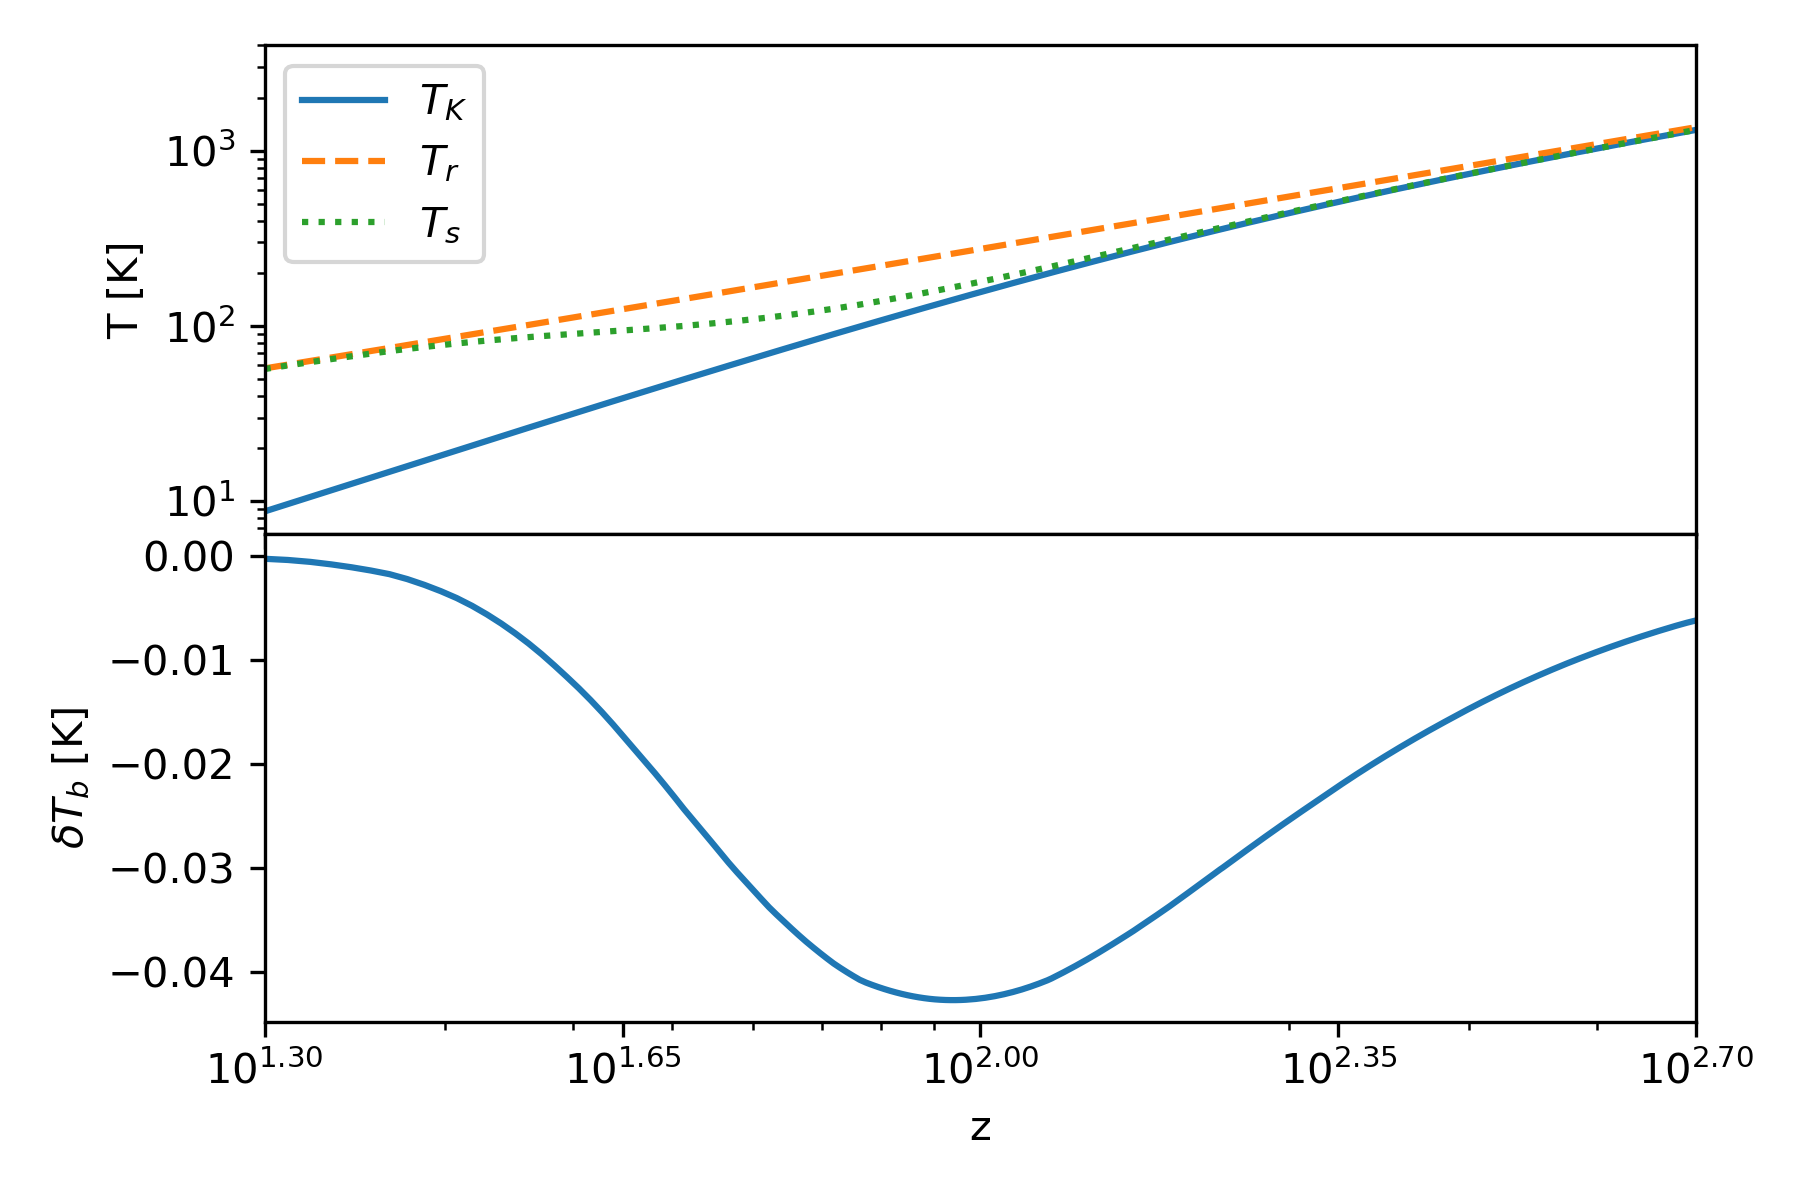
\includegraphics{introduction/figs/example_signal_planck_params.png}
    \caption{The dark ages sky-averaged 21-cm signal. The top panel shows the relationship and evolution of the radio background (orange dashed line), gas temperature (blue solid line) and spin temperature (green dashed line). The bottom panel shows the dark ages 21-cm signal, which is produced by collisional coupling of the spin temperature to the gas temperature. We assume a $\Lambda$CDM baseline \cite{Planck2018}.}
    \label{fig:dark_ages}
\end{figure}

At this early time, collisional coupling drives the spin temperature to the gas temperature, which as just described is lower than the radio background temperature. This produces an absorption feature in the sky-averaged 21-cm signal shown in \cref{fig:dark_ages}. The collisional coupling coefficient is given by
\begin{equation}
    x_c = \frac{\kappa_{10} n_H T_*}{A_{10} T_r},
\end{equation}
where $\kappa_{10}$ is the rate coefficient for spin deexcitations in collisions between neutral hydrogen atoms and is a function of the gas temperature, $T_k$, and $n_H$ is the neutral hydrogen number density. This process is straightforward to model with analytic solutions. Eventually, as the density of the gas reduces, collisions become more infrequent and the spin temperature decouples from the gas and rises back up to the radio background temperature. Collisional coupling will introduce a peak in the 21-cm power spectrum at high-$z$ on scales corresponding to the mean free path for collisions. This all happens prior to the formation of the first galaxies, and a detection of this signal could inform us about key cosmological parameters. The detection of the dark ages signal is the subject of many upcoming missions to the Moon \cite{Burns_Moon_2021} and is not explored significantly in this work.

Once the first stars begin to form around $z\approx25-50$, the spin temperature is expected to couple once again to the gas temperature via the Wouthuysen-Field effect \cite{Wouthuysen1952, Field1959}. In this process, neutral hydrogen atoms absorb and re-emit Lyman-$\alpha$ photons from the first stars which leads to a change in the hyperfine state of the atom and consequently in the spin temperature. The low energy $1_0 S_{1/2}$ hyperfine state, with anti-aligned electron and proton spins, is excited to one of the two central $2P$ states through the absorption of a Lyman-$\alpha$ photon followed by emission and deexcitation to either of the $n = 1$ states. This process is illustrated in \cref{fig:wouthuysen_field}.

The intensity of the Lyman-$\alpha$ emission is driven by the star formation rate in early galaxies. In semi-numerical simulations, the star formation rate is modelled with a star formation efficiency, $f_*$, and the virial circular velocity of star forming halos, $V_c$ \cite{Cohen_global_2017}. The efficiency is the fraction of gas in dark matter halos that is transformed to stars. $V_c$ is then directly related to the halo mass, $M$, via
\begin{equation}
    V_c = 23.4 \bigg(\frac{M}{10^8h^{-1}M_\odot}\bigg)^{1/3} \bigg[\frac{\Omega_m}{\Omega_m^z}\frac{\Delta_c}{18\pi^2}\bigg]^{1/6}\bigg(\frac{1+z}{10}\bigg)^{1/2} \textnormal{km~s}^{-1},
\end{equation}
derived in \cite{Barkana_mass_2001}. Here $M_\odot$ is a solar mass unit, $\Omega_m$ is the matter density parameter, $\Omega_m^z$ is the equivalent as a function of redshift and $\Delta_c$ is the final overdensity relative to the critical density at the collapse redshift of the halo. The effects of varying the astrophysical parameters in the semi-numerical simulations, with a radio background above the CMB, on the global 21-cm signal are shown in \cref{fig:standard_parameters}.

\begin{figure}
    \centering
    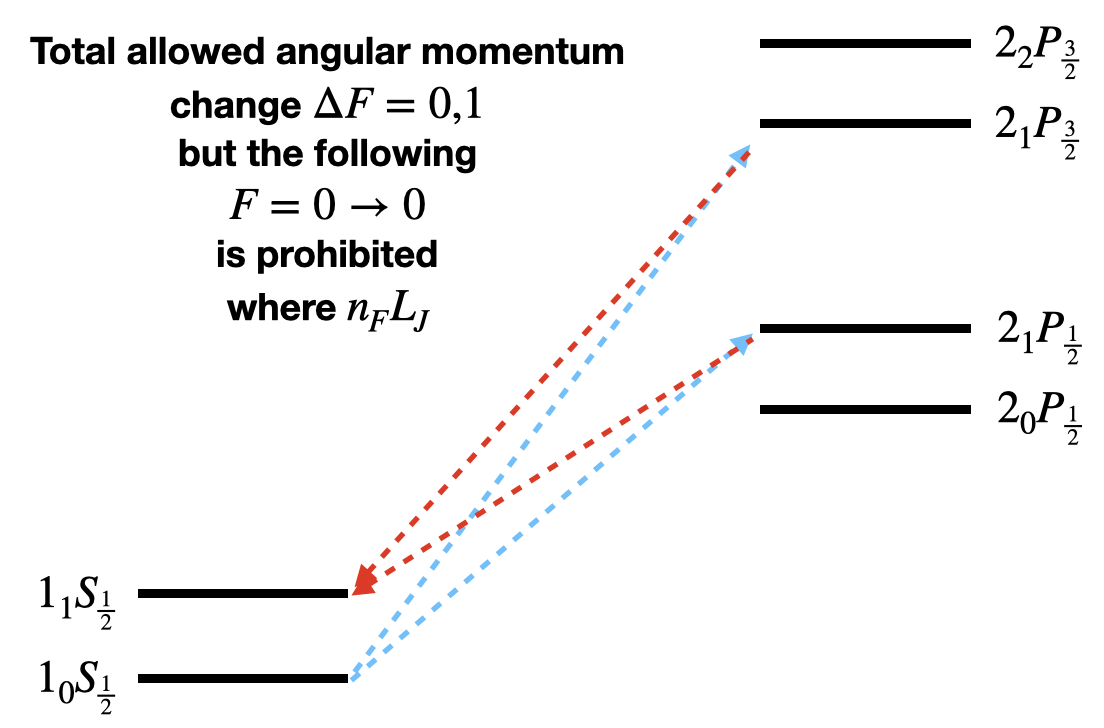
\includegraphics[width=0.8\linewidth]{introduction/figs/Wouthuysen_field.png}
    \caption{The Wouthuysen-Field effect. The absorption and emission of Lyman-$\alpha$ photons by neutral hydrogen drives the spin temperature during the epoch of star formation via the Wouthuysen-Field effect. The blue dashed lines show the absorption of Lyman-$\alpha$ photons and the red show the emission.}
    \label{fig:wouthuysen_field}
\end{figure}

The Wouthuysen-Field effect thus causes an absorption against the radio background between $z\approx20-30$ in the sky-averaged signal, which can be seen in \cref{fig:sky_averaged_signal}, by coupling $T_s$ and $T_k$. In the power spectrum, the Wouthuysen-Field effect manifests itself as a peak at high z and angular scales corresponding to the effective horizon of the coupling process (a few Mpc). In practice, the spin temperature is coupled to the colour temperature, $T_{c}$, but since the IGM is optically thick to Lyman-$\alpha$ emission during this period $T_c \approx T_k$. The coupling coefficient is given by
\begin{equation}
    x_\alpha = \frac{4 P_\alpha T_*}{27 A_{10} T_r},
\end{equation}
where $P_\alpha$ is the total rate at which Lyman-$\alpha$ photons are scattered per atom. $x_\alpha$ is directly proportional to the angular averaged intensity of Lyman-$\alpha$ emission, $J_\alpha$, via $P_\alpha$. During this epoch $T_k$, and the coupled spin temperature, continues to cool at a faster rate than the radio background. However, various heating processes begin when the first stars begin to form raising the gas temperature and preventing $T_k$ from cooling adiabatically. These include Lyman-$\alpha$, X-ray, CMB and shock heating.

\begin{figure}
    \centering
    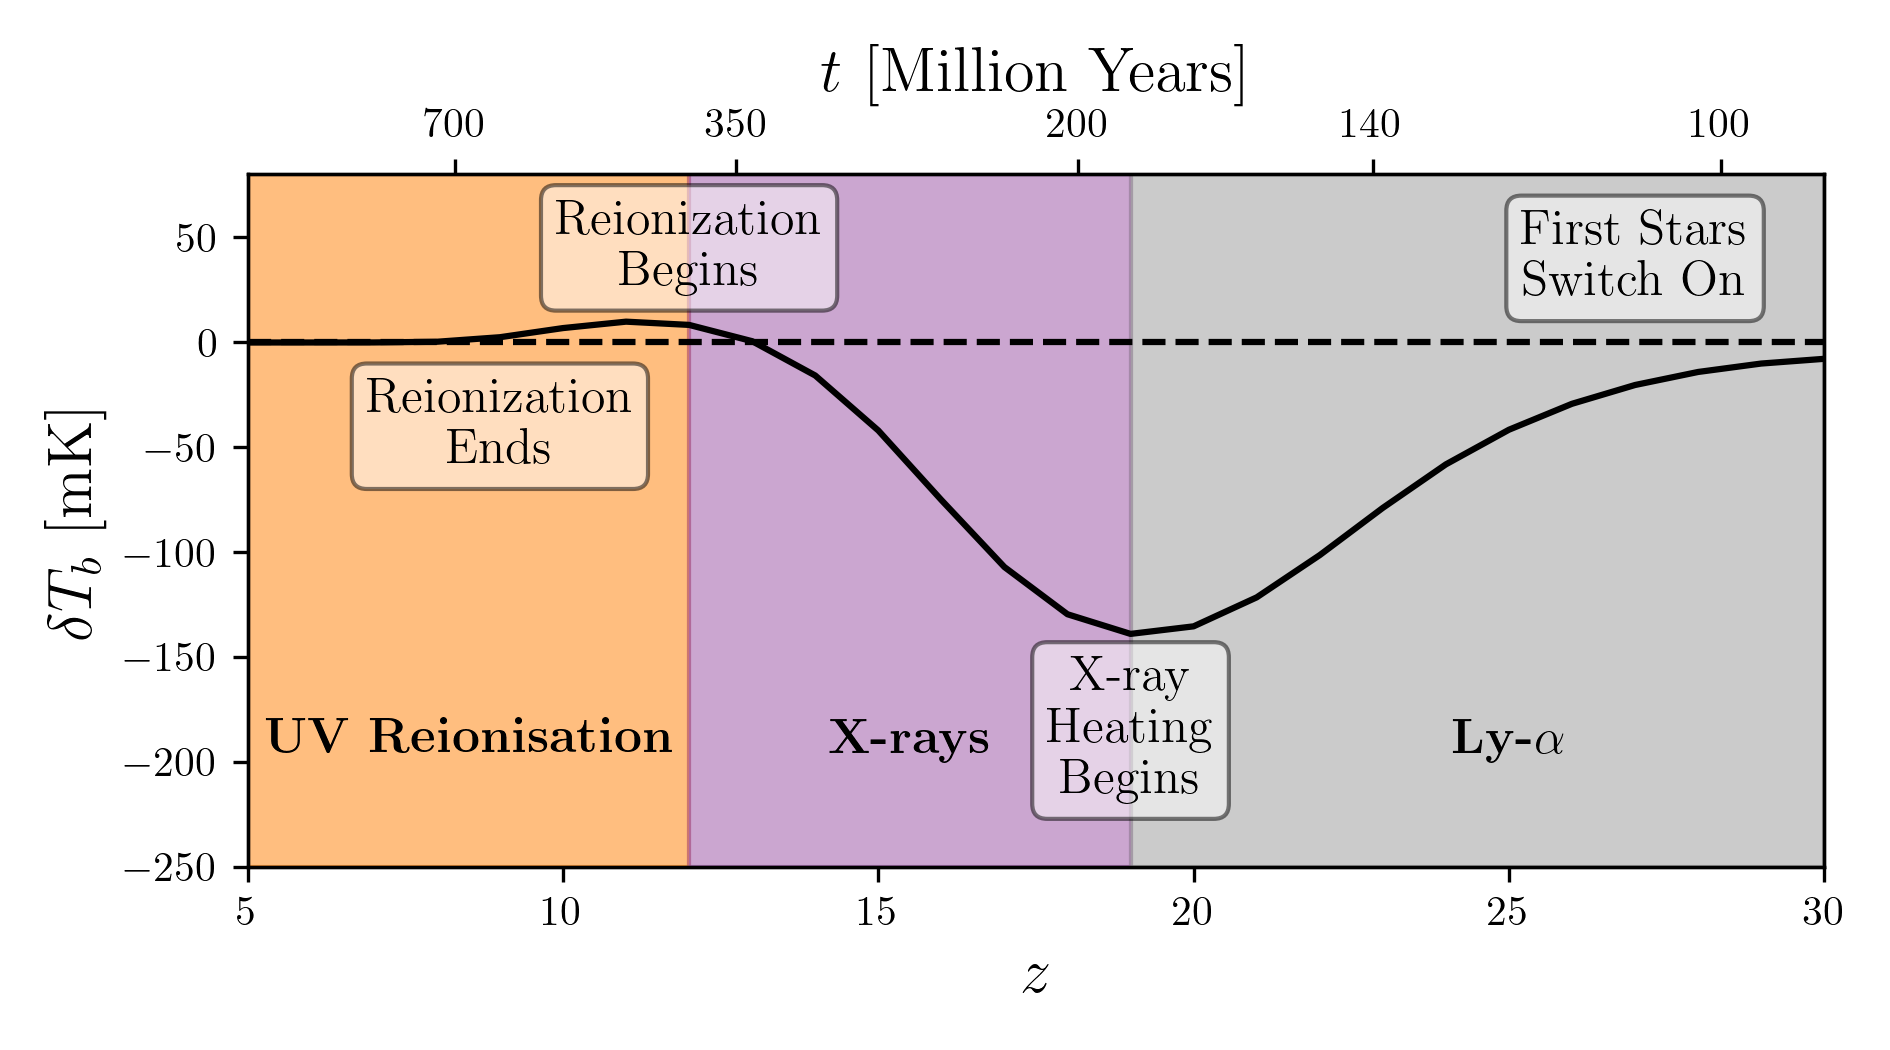
\includegraphics{introduction/figs/signal.png}
    \caption{The 21-cm signal from the Cosmic Dawn and Epoch of Reionization is highly dependent on the intensity of a number of different radiative fields. The figure illustrates the dominant radiative fields as a function of redshift and time after the Big Bang and as a backdrop to an example 21-cm signal. At early redshift, when the first stars switch on, Lyman-$\alpha$ emission drives the spin temperature to the gas temperature, causing an absorption in the signal against the radio background. CMB and Lyman-alpha heating begin to play an important role in modulating the gas temperature and then at later redshifts along with X-ray heating raise the gas temperature back up to and sometimes beyond the radio background temperature. Finally, at more recent times and low redshifts UV emission from stars ionizes the neutral hydrogen and the signal disappears against the radio background. The signal shown here was generated with the neural network signal emulator \textsc{globalemu}, which is discussed in \cref{ch:globalemu}, trained on simulations with a radio background equivalent to the CMB.}
    \label{fig:sky_averaged_signal}
\end{figure}

Lyman-$\alpha$ heating plays a significant role in determining the structure of the global 21-cm signal \cite{Reis_sta_2021}. This mechanism deposits energy in the gas, increasing $T_k$, via the scattering of Lyman-$\alpha$ photons, that induce the Wouthuysen-Field effect, and although the energy deposited per event is small the number of scattering events is large. Since $T_k$ and $T_s$ are coupled at this time, both begin to move back towards the radio background temperature, reducing $\delta T_b$. The Wouthuysen-Field effect still dominates during this period but the heating mechanism significantly reduces the maximum allowed theoretical depth of the global signal from $\approx - 250$~mK to $\approx - 165$~mK \cite{Reis_sta_2021} assuming the radio background is equal to the CMB temperature. This process begins as soon as the first stars form, whereas X-ray heating is delayed until quasars and X-ray binaries begin to form. The heating mechanisms in general suppress the low-$z$ power spectrum peak induced by the Wouthuysen-Field effect \cite{Chuzhoy2007, Villanueva2020, Venumadhav2018, Reis_sta_2021, Mittal2021}.

\begin{figure}
    \centering
    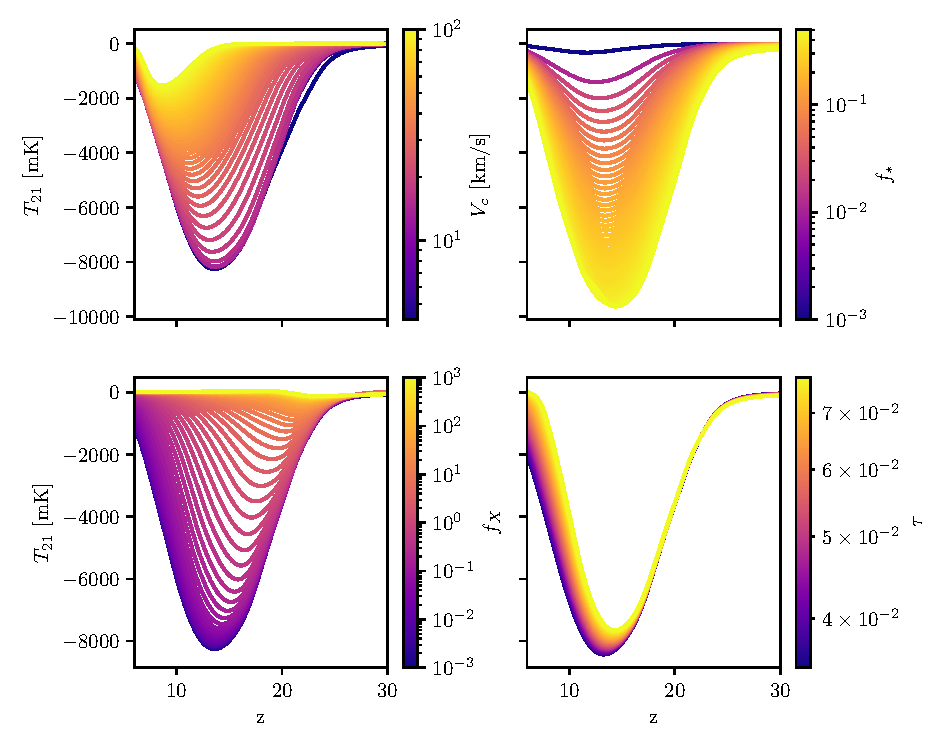
\includegraphics{introduction/figs/other_params_variation.pdf}
    \caption{The figure shows the effect of varying four different parameters of the semi-numerical simulation detailed in the text and throughout this thesis. The base signal that is varied has strong star formation, inefficient X-ray heating and a strong radio background. The simulations have an excess radio background above the CMB from high redshift radio galaxies. The minimum virial circular velocity, $V_c$, and the star formation efficiency, $f_*$, determine the star formation rate and consequently the Lyman-$\alpha$ flux. Low values of $V_c$ and high values of $f_*$ lead to high Lyman-$\alpha$ fluxes, strong coupling between the spin temperature and the gas temperature, and as a result deep 21-cm signals. It also influences the onset of heating, however this is harder to disentangle from X-ray heating. X-ray heating is governed by the X-ray efficiency, $f_X$, in these simulations. Low values of $f_X$ lead to inefficient X-ray heating and push the minimum of the global 21-cm signal down and to lower redshifts. Finally, we show the variation in the signal with the CMB optical depth, $\tau$, which has very little influence in the structure of the signal at high redshift but becomes more important at low redshift during the Epoch of Reionization. It's important to note that these effects are not independent and do not occur at distinct epochs but rather overlap, meaning that the structure of the signal as a function of redshift is complex. However, figures like this help to gain an intuition for how each parameter affects the structure of the signal. Again, the signals were produced with the neural network emulators discussed primarily in \cref{ch:globalemu} and then also in \cref{ch:saras2} and \cref{ch:saras3}.}
    \label{fig:standard_parameters}
\end{figure}

A related heating mechanism is CMB heating, in which energy is transferred from the radio background to the gas via interactions with neutral hydrogen. In CMB heating, a CMB photons raise the energy state of the electron in the neutral hydrogen atom from $1_0$S$_{1/2}$ to $1_1$S$_{1/2}$ and the neutral hydrogen atom subsequently scatters with a Lyman-$\alpha$ photon. The scattering raises the electron into one of the 2P states and then the electron can deexcite back into the $1_0$S$_{1/2}$ releasing a higher energy Lyman-$\alpha$ photon in the process. The additional energy has come from the CMB photon and is transferred by the Lyman-$\alpha$ photon to the gas thus raising the gas temperature~\cite{Venumadhav2018}. CMB heating can reduce, $x_r$ which is dependent on the 21-cm optical depth
\begin{equation}
    x_r = \frac{1 - \exp(-\tau_\nu)}{\tau_\nu},
\end{equation}
below 1 \cite{Reis_sta_2021}.

Further heating occurs through IGM shocks. As the Universe expands the density fluctuations seen in the CMB grow to form galaxies and large scale structure. However, these density fluctuations are not spherical and so collapse into sheets or ``Zel'dovich pancakes'', filaments and halos. During this process of collapse, if the velocity of the infalling gas is higher than the speed of sound, some of the gravitational infall energy is transformed into thermal energy via shocks. Shocks are only important when the temperature of the shock, $T_\mathrm{sh}$, is greater than $T_k$ and the temperature scales as the mass of the collapsing region to the power of six. The process plays a more significant role at high redshift but the energy transferred to the IGM through shocks reduces with increasing time and is generally thought to be minimal throughout the CD and EoR \cite{Furlanetto_review_2006, Mesinger2019}.

Finally, X-ray heating plays a significant role in the structure of the global 21-cm signal. It produces a peak in the power spectrum as a function of redshift and at the relevant galactic and intergalactic scales. X-ray heating is expected to begin around redshifts 15-20. Low energy X-rays and some high energy X-rays with long mean free paths from Galaxies and quasars are absorbed by the IGM and deposit most of their energy as kinetic energy raising the gas temperature, $T_k$, which at this time is still coupled to the spin temperature via the Wouthuysen-Field effect. Further, the X-rays photoionize hydrogen and helium in the IGM with the resulting free electrons retaining the majority of the photon energy as kinetic energy. This kinetic energy is subsequently deposited into the IGM via collisional ionization and excitation of helium and hydrogen. Collisional ionization leads to a background of secondary electrons that subsequently deposit kinetic energy into the IGM and excitation of helium creates a background of photons that go on to ionize hydrogen. Collisional excitation of hydrogen in turn produces a background of Lyman-$\alpha$ photons which can heat the gas through the process described above. Finally, the free electrons created by X-ray photoreionization of hydrogen can heat the IGM through Compton collisions with other free electrons.

The high redshift X-ray background is poorly understood and in the semi-numerical simulations employed throughout this thesis it is assumed that the relationship between the X-ray luminosity and the star formation rate at low redshifts can be extrapolated, taking into account an increase in luminosity with decreasing metallicity, to high redshifts. Between 0.2 - 10 keV the luminosity is given by
\begin{equation}
    L_X = 3\times 10 ^{40} f_X \bigg(\frac{\mathrm{SFR}}{1 M_\odot \mathrm{yr}^{-1}}\bigg) \mathrm{erg~s}^{-1},
\end{equation}
where $f_X$ is the efficiency of X-ray production in high redshift galaxies, effectively acting as a normalisation parameter, and a free parameter in our models. We model the spectrum of X-ray sources in the simulations under the assumption that they are predominantly X-ray binaries in which stellar mass from a main sequence star accretes onto a neighbouring compact object. These systems should be prominent in the early Universe and should form as the first population of stars begins to die. We characterise the spectra of the X-ray binaries either empirically from \cite{Fragos_Xrays_2013} or analytically with two free parameters in our semi-numerical simulations; $\nu_\mathrm{min}$ (occasionally referred to $E_\mathrm{min}$) which is the low energy cut-off of the spectral energy density and $\alpha$ which is the slope of the spectral energy density. %The modelling of the X-ray background is limited and additional contributions from for example quasars are not included, however it is expected to be sufficient for current requirements. 
In some instances, X-ray heating can be sufficiently large to raise the gas temperature and coupled spin temperature above the radio background temperature, as can be seen in \cref{fig:sky_averaged_signal}.

At lower redshifts, reionization, in which neutral hydrogen is ionized via UV emission from the first stars, begins to dominate the structure of the 21-cm signal during the Epoch of Reionization. Once all the hydrogen is ionized and the neutral fraction of hydrogen in \cref{eq:bright_temp}, $x_{HI} = 0$, then the signal disappears against the radio background. Reionization occurs first around the sources of UV emission and is dependent on the mean free path, $R_\mathrm{mfp}$, of the ionizing radiation which is a free parameter in the semi-numerical simulations. The total column density of the ionizing gas is measured by the CMB optical depth $\tau$ which is proportional to the ionizing efficiency of sources, $\zeta$. Again, $\tau$ is a free parameter in the simulations. It has previously been constrained by Planck, however, its value remains uncertain with a strong dependence on the reionization model. The 21-cm line offers an alternative means by which it can be constrained. UV reionization begins as soon as the first stars form and UV photons in the Lyman-Werner band deplete the amount of neutral hydrogen that can go into stars via ionization thus suppressing star formation in a process known as Lyman-Werner feedback \cite{Cohen_global_2017}. However, the strength of this feedback mechanism is not well understood \cite{Visbal_lw_2014}.

Typically, the radio background in simulations of the 21-cm signal is set to the CMB temperature. However, we know that radio galaxies should contribute to this background. Further, measurements from the balloon experiment Absolute Radiometer for Cosmology, Astrophysics, and Diffuse Emission~(ARCADE2) \cite{fixsen_arcade_2011} and the Long Wavelength Array~(LWA) \cite{dowell_radio_2018} suggests that there is a radio background in excess of the CMB which can be modelled as a homogeneous synchrotron source. However, there are concerns about the galactic modelling in the two experimental measurements of the excess \cite{Subrahmanyan2013}. The reported detection from the EDGES experiment in 2018 also hints at the possibility of an excess radio background, however there are concerns about the modelling of the EDGES data (see \cref{sec:current_results}). A larger radio background leads to a stronger contrast with the spin temperature and consequently a deeper absorption feature in the global 21-cm signal and a larger power spectrum.

\begin{figure}
    \centering
    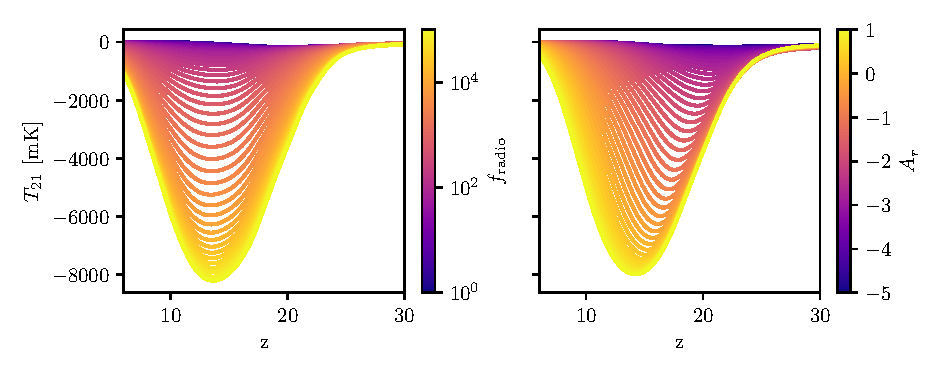
\includegraphics{introduction/figs/backgrounds_variation.pdf}
    \caption{The figure shows the variation of two different parameterisations of  exotic global 21-cm signals with excess radio backgrounds. In both figures the star formation rate is high (with a high star formation efficiency and low minimum virial circular velocity) and the X-ray efficiency is low, which along with a large radio background produces a deep signal. The CMB optical depth is set to 0.05 and its value is only important at low redshifts. The left-hand panel corresponds to an excess radio background above the CMB produced from radio galaxies and mediated by the radio production efficiency, $f_\mathrm{radio}$, which is proportional to the radio luminosity per star formation rate, $L_r/\mathrm{SFR}$. The right-hand panel corresponds to an excess from a homogeneous synchrotron source and its magnitude is mediated by $A_r$ which is effectively the fractional increase on the CMB at a given frequency (here 78 MHz). The excess radio background models were originally proposed to explain the anomolously deep EDGES absorption feature reported in 2018. More details can be found in the text. The signals were generated using the neural network emulator detailed in \cref{ch:globalemu}, \cref{ch:saras2} and \cref{ch:saras3}.}
    \label{fig:radio_parameters}
\end{figure}

Throughout the later chapters of this thesis, we use semi-numerical simulations with two different parametrisations of an excess (over the CMB) radio background. The first is from a synchrotron source which produces a uniform radio background
\begin{equation}
    T_\mathrm{r} = T_\mathrm{CMB}\bigg[ 1 + A_{\mathrm{r}}^{78}\bigg(\frac{\nu}{78\textnormal{MHz}}\bigg)^\beta\bigg],
    \label{eq:srb_background}
\end{equation}
that decays with increasing time. Here $A_r$ is a fractional increase on the CMB at a given frequency, and it can be scaled according to
\begin{equation}
    A_{\mathrm{r}}^{78} = A_{\mathrm{r}}^{1420} \bigg(\frac{0.078}{1.420}\bigg)^\beta,
\end{equation}
where $\beta$ is often chosen to be equal to $-2.6$ consistent with measurements from ARCADE2 and LWA. This model has a larger impact on the global 21-cm signal at higher redshifts and generally pushes the minimum of the global 21-cm signal to higher redshifts which can be seen in \cref{fig:radio_parameters}. The synchrotron excess may be sourced by superconducting cosmic strings \cite{Brandenberger2019} or light dark matter decays \cite{Fraser2018, Pospelov2018}. Since the radio background is homogeneous, it leads to an increase in the power spectrum at all angular scales, but its impact is again more significant at high redshifts.

The second parameterisation of the radio background is from high redshift radio galaxies. In this instance the radio background is modelled via the radio production efficiency, $f_\mathrm{radio}$, which is proportional to the radio luminosity per star formation rate
\begin{equation}
L_r	= 10^{22} f_\mathrm{radio} \bigg(\frac{\nu}{150~\mathrm{MHz}}\bigg)^\beta \bigg(\frac{\mathrm{SFR}}{M_\odot~\mathrm{yr}^{-1}}\bigg)~\mathrm{W~Hz}^{-1},
\end{equation}
where again $\beta$ is usually set to $-2.6$. The level of excess background above the CMB in this model increases with decreasing redshift, in contrast to the previously discussed model, as more radio galaxies form. It is also non-uniform unlike the synchrotron model. This non-uniformity leads to an increase in the power spectrum on angular scales corresponding to galactic and intergalactic length scales. The model has a similar effect on the depth of the global 21-cm signal to the synchrotron model creating a stronger contrast between $T_s$ and $T_r$. However, as can be seen in \cref{fig:radio_parameters}, it does not affect the redshift of the minima in the global signal.

Since the 21-cm signal is highly dependent on the amplitude of a number of different radiation fields, it is a powerful probe of the infant Universe and the first galaxies. Its detection represents one of the final frontiers in observational cosmology, along with studies of dark energy, dark matter and gravitational waves. In the later chapters of this thesis, we present the current best limits on the properties of early galaxies from 21-cm cosmology, but presently we describe the challenges of making a detection.

\section{Challenges facing the field}

There are a number of different challenges facing the field of 21-cm cosmology, and we detail several specific issues in the following subsections. This is followed by a more general discussion of `unknown systematics' in which we group together additional challenges that if incorrectly dealt with can introduce non-smooth structure into the data that mimics, corrupts or hides the global 21-cm signal. We focus on the detection of the sky-averaged 21-cm signal here, as that is the main focus of the thesis, but note that there are similar challenges and unique problems in studies of the power spectrum.

\subsection{Galactic, extra-galactic foregrounds and the antenna beam}
\label{sec:foregrounds}

Radiometers aiming to detect the sky-averaged 21-cm signal also pick up emission from the Galaxy and from other galaxies, which dominates over the order $100$~mK cosmological signal. This foreground is composed of synchrotron and free-free emission and is approximately five orders of magnitude larger than the 21-cm signal, as can be seen in \cref{fig:relative_signal_magnitudes}. The foregrounds are expected, from the theory of synchrotron and free-free emission, to be smooth and follow an approximate $\nu^{-2.5}$ power law. SARAS3 found that the sky had a spectral index of $-2.42$ \cite{SARAS3}, EDGES found it to be approximately $-2.6$ as a function of local sidereal time \cite{Mozdzen_EDGES_spectral_index_2017}, and LEDA reported a measurement of the spectral index to be $\beta = -2.5 \pm 0.1$ \cite{LEDA_spectral_Index_2021}.

\begin{figure}
    \centering
    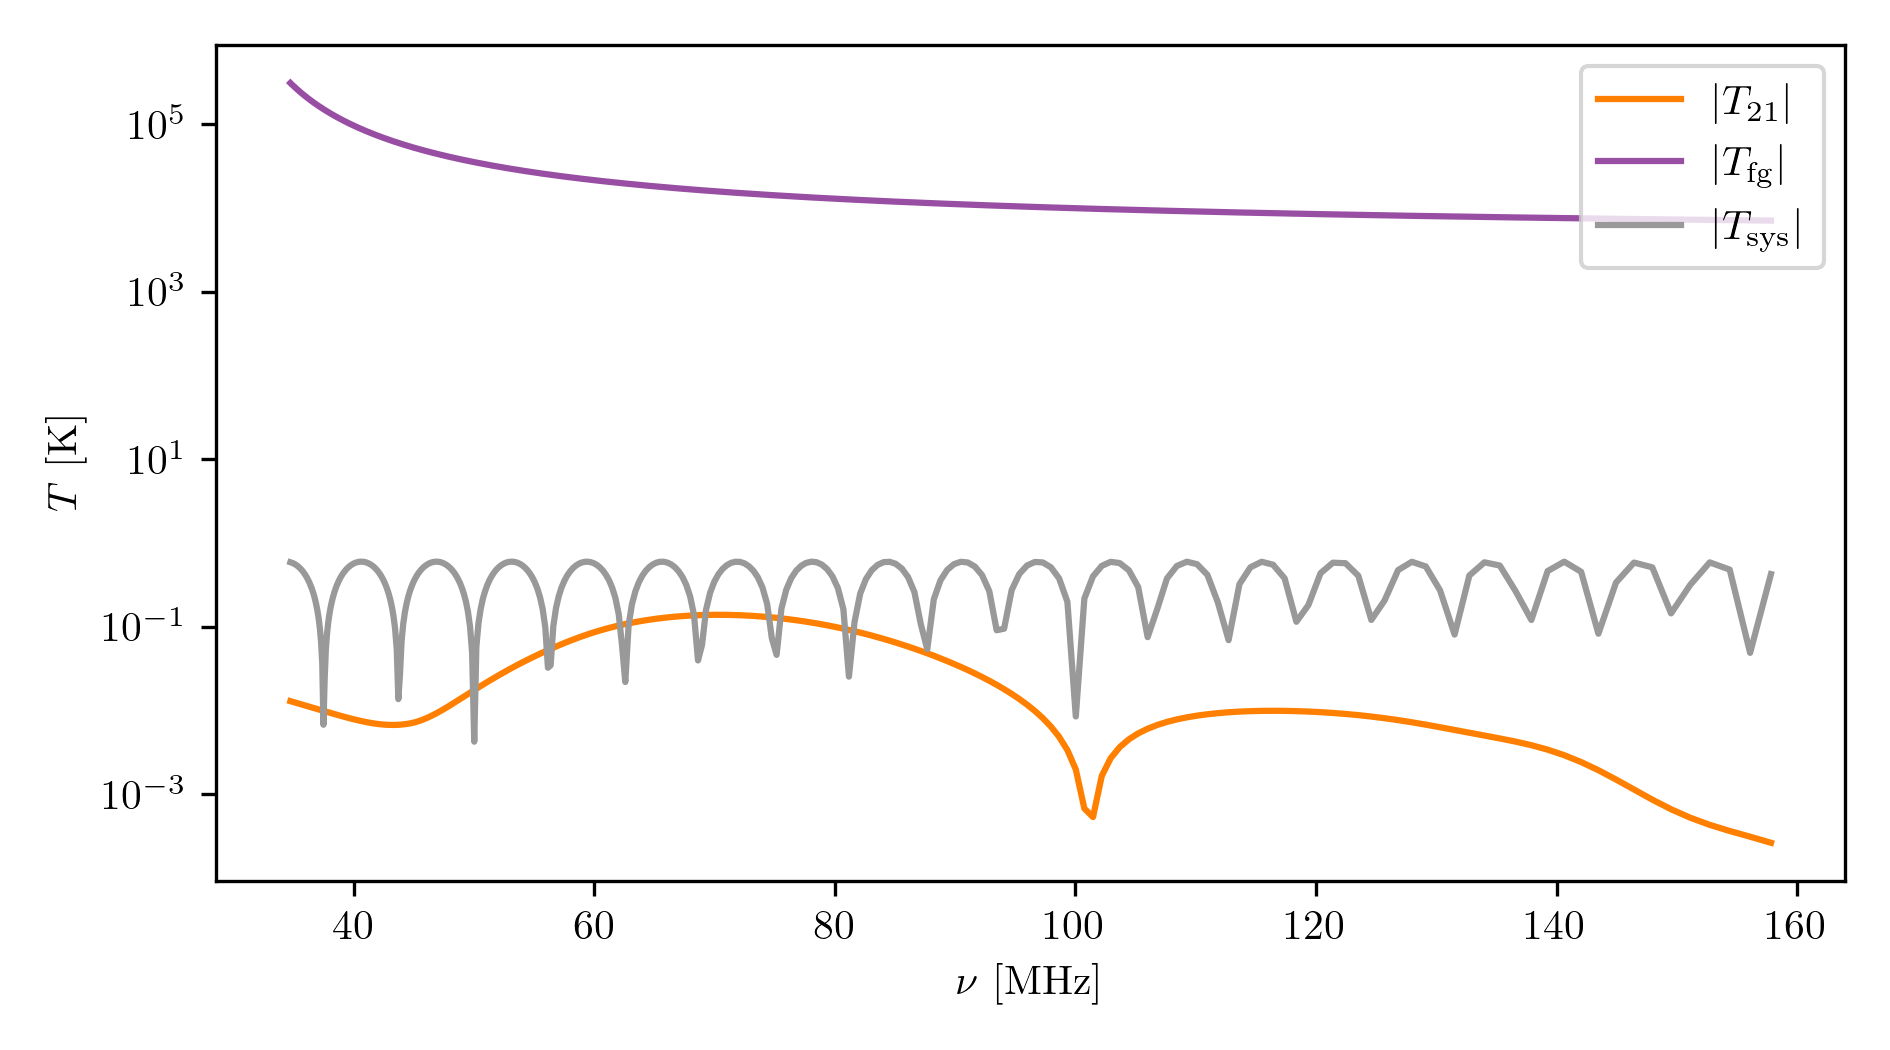
\includegraphics{introduction/figs/the_data.png}
    \caption{The graph shows the relative magnitude of different signals collected by global 21-cm experiments. The foregrounds (purple) are around five orders of magnitude larger than the 21-cm signal (orange). Sinusoidal systematics are frequently found in the data from these experiments and can be caused by cable reflections, chromaticity in the beam and discontinuities in the soil among other things discussed in the text. We show an example systematic (grey) to illustrate that these signals have similar magnitudes to the 21-cm signal and need to be corrected for.}
    \label{fig:relative_signal_magnitudes}
\end{figure}

Since the foreground dominates so significantly over the 21-cm signal, it is essential that the two signals can be separated from each other. To do this, we often take advantage of the fact that the foreground is smooth, and the signal is not over a wide frequency (or equivalently redshift) range. The idea is that we model the smooth structure in the data with a low order polynomial function, often in log-space,
\begin{equation}
    \log_{10}T_\mathrm{fg}(\nu) = \sum_i^N a_i \log_{10}(\nu)^i,
\end{equation}
where the coefficients $a_i$ are fitted for, to leave behind the non-smooth 21-cm signal. Alternative physically motivated polynomial models have also been proposed, however their applications have been limited \cite{Bowman_edges_2018}.

There are however complications with the principle of separating smooth foregrounds from the non-smooth signal with polynomials. It requires the design of a wideband instrument, since over narrow frequency ranges the 21-cm signal is also smooth and easily modelled by low order polynomials. Whilst designing a wideband antenna is possible, this leads to a very non-smooth response from the antenna to the sky, which can be difficult to correct for. This effect in the antenna beam is known as chromaticity and is a major issue for 21-cm experiments.

In \cref{fig:chromaticity}, we illustrate how the structure of the antenna beam affects the recorded data. We use an elliptical dipole above an infinite ground plane shown in the bottom right of the figure to illustrate, along the top row, how a slice through the beam at a fixed azimuthal angle changes with frequency from $50 - 200$~MHz. We then posit the existence of two bright sources in the sky, shown by the purple and orange stars, which have smooth spectra that are power laws in frequency with $\beta \approx -2.5$ as shown by the orange and purple dashed lines in the figure on the bottom left. The incoming radiation from these two bright sources is effectively along the line of sight because they are so distant that radial emission is not seen by the antenna.

\begin{figure}
    \centering
    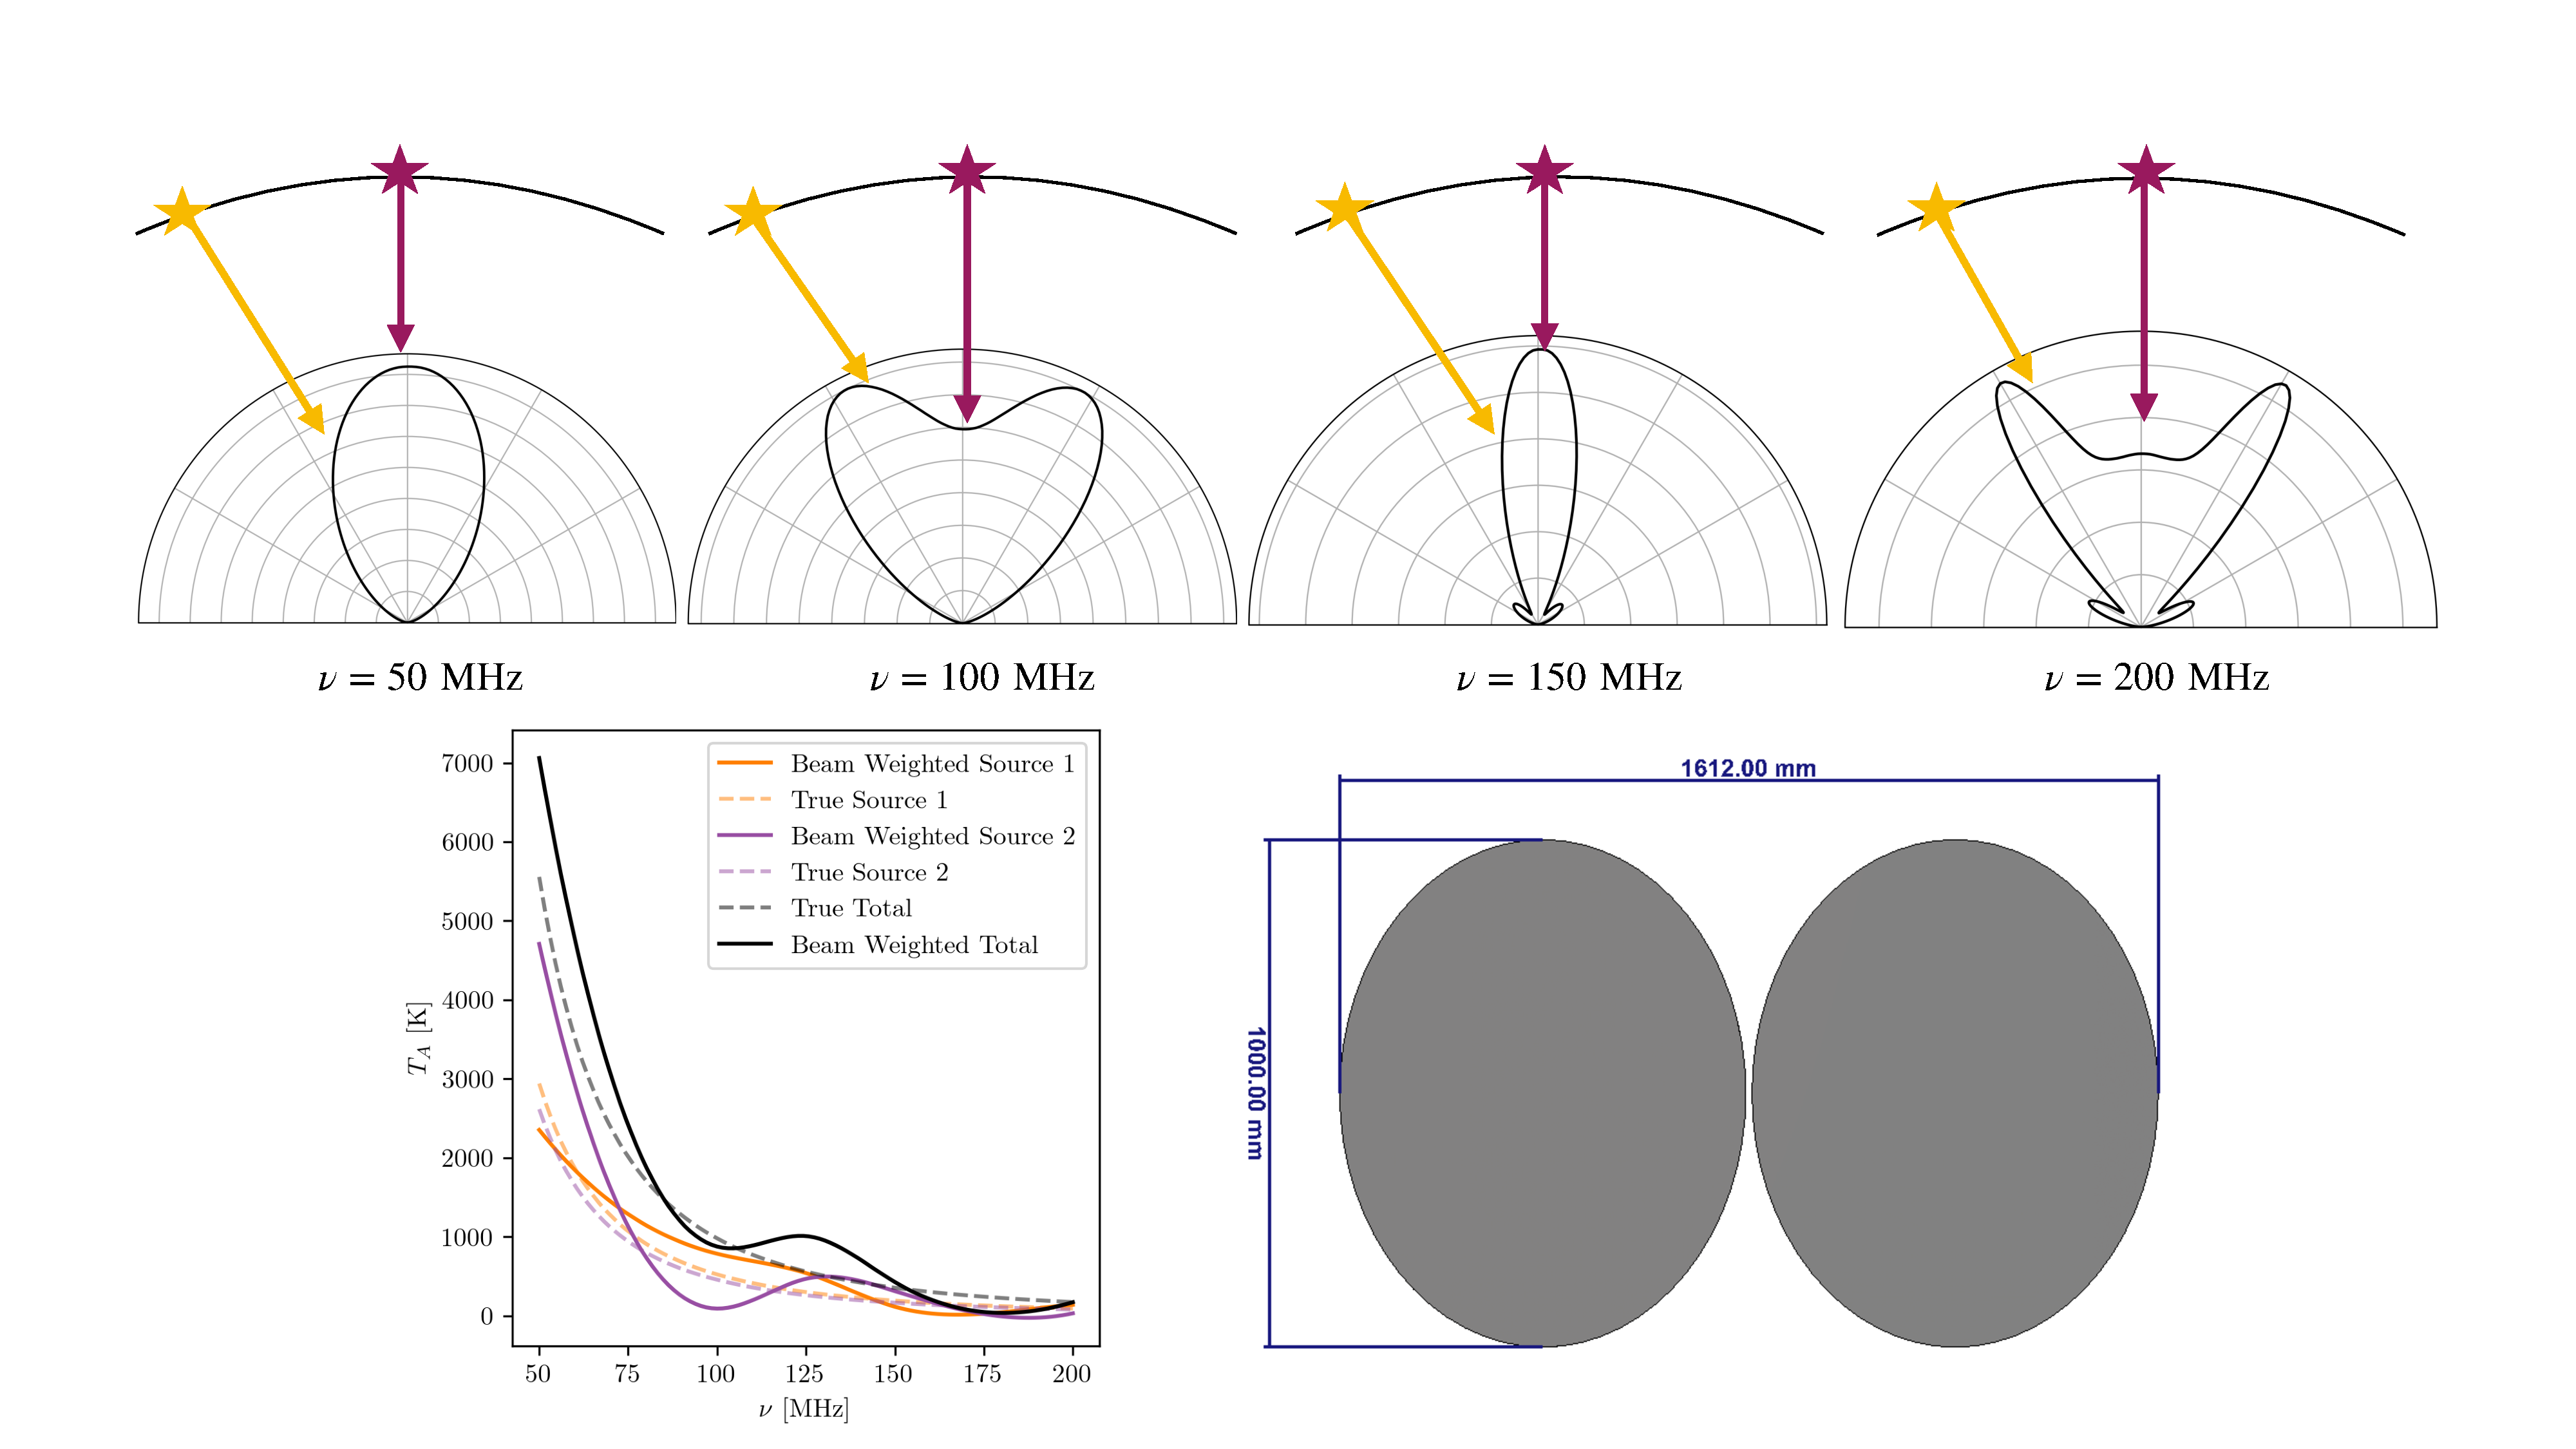
\includegraphics[width=\linewidth]{introduction/figs/chromaticity.pdf}
    \caption{The figure illustrates the impact of a chromatic beam on the sky-averaged 21-cm signal. The bottom right panel shows a Computer Simulation Technology~(CST) model of an elliptical dipole antenna, provided by Dominic Anstey and John Cumner. Along the top row, we show slices through the beam at four fixed frequencies in the range of interest for a 21-cm experiment. The structure of the beam changes with frequency and this causes signals from the sky to be down-weighted at some frequencies relative to others. To illustrate this, we show two different point sources, which we assume to have approximate power law spectra, and how they interact with the beam. The bottom left-hand panel shows the ``true spectrum'' for each source as dashed lines and the recorded spectra as solid lines. We also show the sum of these two point source spectra in black. The beam introduces significant non-smooth structure into the data and this needs to be appropriately modelled so that the 21-cm signal can be recovered from the data. In practice, the problem is much more complicated because the beam is three-dimensional, the sky is full of complex structure and the sky varies with time.}
    \label{fig:chromaticity}
\end{figure}

The beam weights the input power from the sky, $T_\mathrm{sky}$, based on its directivity which as can be seen in the top row is a function of angle and frequency. The solid orange and purple lines in the bottom left panel show the weighted spectra which feature chromatic distortion, where the weighting has been exaggerated for demonstration, from the two posited point sources. This can also be seen in the sum of the spectra, shown in black.

In practice, the problem is much more complicated because the beam is 3D, the sky is rich in complex structures such as the galactic plane, the north galactic spur and bright sources such as Cygnus A, and observations are taken over long periods in which the sky rotates above the beam. However, from the simple example we can clearly see how the beam can introduce non-smooth structure into the antenna temperature, $T_A$, and how modelling the foreground in wideband data with a smooth low-order polynomial will leave behind both the non-smooth signal but also a large non-smooth chromatic residual.

One approach to deal with chromaticity is to fit high order polynomials in an effort to model the foreground and the non-smooth chromatic structure in the data. However, this can of course fit out the 21-cm signal as well.

More complete approaches to modelling the effects of chromaticity can be taken. For example, the EDGES collaboration \cite{Mozdzen_EDGES_spectral_index_2017} proposed a correction given by
\begin{equation}
    B(\nu, t) = \frac{\int_\Omega T_\mathrm{sky-model}(\nu_\mathrm{ref}, t, \theta, \phi) D(\nu, \theta, \phi) d\Omega}{\int_\Omega T_\mathrm{sky-model}(\nu_\mathrm{ref}, t, \theta, \phi) D(\nu_\mathrm{ref}, \theta, \phi) d\Omega},
\end{equation}
where $D$ is the directivity of the antenna, $t$ is the time, and $\theta$ and $\phi$ are the zenith and azimuthal angles parameterising the beam. The sky temperature is modelled by the difference between a map and the CMB scaled by a signal power law
\begin{equation}
    T_\mathrm{sky-model} (\nu_\mathrm{ref}, t, \theta, \phi) = [T_\mathrm{base-map} - T_\mathrm{CMB}]\bigg(\frac{\nu_\mathrm{ref}}{\nu_\mathrm{base-map}}\bigg)^{-2.5}.
\end{equation}
The corrected antenna temperature is then given by
\begin{equation}
    T_\mathrm{cor} = \int_{t_\mathrm{start}}^{t_\mathrm{end}} \frac{T_\mathrm{data} - T_\mathrm{CMB}}{B} dt + T_\mathrm{CMB}.
\end{equation}
However, this correction assumes an exact knowledge of the foreground and the antenna beam pattern. In practice the foreground maps are not known well enough and while we can model the antenna beam it is difficult to account fully for the environment around the antenna and for imperfections in manufacturing.

A sophisticated forward modelling of the antenna beam and the foreground has been proposed in a series of papers \cite{Anstey_REACH_2021, Anstey_antenna_2022, Anstey_lst_2022}. The model uses a base sky map which is divided into $N$ regions of varying spectral index and convolved with a model of the beam
\begin{equation}
    T_\mathrm{fg} = \frac{1}{4\pi}\int_0^{4\pi} D(\nu, \theta, \phi) \int_{t_\mathrm{start}}^{t_\mathrm{end}} \sum_{i=0}^{N} M_{i}(\theta, \phi)[T_\mathrm{base-map} - T_\mathrm{CMB}]\bigg(\frac{\nu}{\nu_\mathrm{base-map}}\bigg)^{-\beta_i} dt d\Omega + T_\mathrm{CMB},
\end{equation}
where $M_i(\theta, \phi)$ is the mask that divides the sky map into $N$ regions of identical spectral index $\beta_i$. Work is currently ongoing on a model for any deviation in the beam from the simulations caused by environmental and manufacturing errors.

Ground plane artefacts can be introduced in the data by finite edges or discontinuities in the structure, which are usually hard to model \cite{Bradley_EDGES_2019}. These can produce standing waves on the finite edges of the ground plane and introduce ripples that are unaccounted for in the modelling of $D(\nu, \theta, \phi)$. Ground planes are typically employed for dipole antennas to prevent the antenna looking at the ground with the same efficiency that it looks at the sky, however emission from the soil can still cause problems and discontinuities in the soil structure can also distort the directivity of the antenna.

The 21-cm signal is also affected by chromaticity, but the foregrounds change on much larger length scales and the intensity of the foregrounds vary much more across the sky. We can therefore generally ignore chromatic effects in the sky-averaged 21-cm signal.

Power spectrum experiments also struggle with the effects of the antenna beams and the foregrounds. For example, a major cause of systematics in these experiments is cross-talk between different antennas in the interferometric array. Cross-talk occurs because antennas re-radiate reflected signals, and this can be picked up by neighbouring antennas in the often closely packed array. A detailed discussion of the systematics in power spectrum experiments and how these experiments deal with foregrounds is beyond the scope of this thesis. Briefly, however, one of the most effective ways of dealing with foregrounds in power spectrum experiments takes advantage of the fact that the foreground and 21-cm signals appear on different angular scales and different redshifts meaning that the foregrounds can be avoided by looking at small angular scales at late times. 

In global or sky-averaged experiments we can try to avoid chromatic effects, however, this is very difficult even with a narrowband instrument. Such antennas have frequency independent beams and are known as achromatic antennas. Currently, there is only one collaboration, SARAS, attempting to build such antennas. They are relying on monopole antennas and observing over narrow bandwidths. 

It has been shown via simulations that the SARAS2 instrument has an approximately achromatic response to the sky over the redshift range $z\approx7-12$ \cite{Sathyanarayana_msf_2017}. However, as shown in \cref{ch:saras2} the data features sinusoidal systematics which were likely introduced by discontinuities in the ground below the antenna setting up a standing wave in the beam pattern which was not modelled and introduced chromaticity. In contrast, the SARAS3 instrument was situated on a lake and the data was found to be smooth and absent of chromatic structure over the observing band $z\approx15-25$ (see \cref{ch:saras3}). 

Polynomial foreground models remain a useful tool if we can build and collect data with a perfectly achromatic beam. However, they can still fit out the 21-cm signal if the order is too high. This can be overcome by forcing the polynomial to be smooth by constraining the coefficients of the model so that the higher order derivatives do not cross zero
\begin{equation}
    \frac{\delta^m T_\mathrm{fg}}{\delta \nu^m} \leq 0~~\mathrm{or}~~ \frac{\delta^m T_\mathrm{fg}}{\delta \nu^m} \geq 0.
\end{equation}
Such polynomials are called `Maximally Smooth Polynomials' and were originally proposed in \cite{Sathyanarayana_msf_2017} and \cite{Sathyanarayana2015}. They are the subject of \cref{ch:maxsmooth}, where we expand the definition to the more general `Derivative Constrained Functions'~(DCFs) and introduce an efficient fitting algorithm for this non-trivial problem.

In principle, DCFs should leave behind the non-smooth signal in the residuals and indeed will leave behind any non-smooth previously unexpected chromatic residuals in the data. The application of DCFs is of course still subject to the issue of narrowband observations of smooth sections of the 21-cm signal.

\subsection{The atmosphere}

The atmosphere also poses a problem for observations of the global 21-cm signal, and in particular the ionosphere, which is an ionized layer of the atmosphere between $\approx 50 - 1000$~km above sea level. As radio waves propagate through this layer of the atmosphere they can be absorbed and refracted with the effect being more severe for lower frequencies (scaling as $\nu^{-2}$)\cite{Vedantham_ionosphere_2014, Datta_ionosphere_2014, Shen_ionosphere_2021}. The ionosphere is subdivided into multiple layers in which propagating radio waves are modulated in different ways.

The refraction of the radio waves in the F-layer of the ionosphere distorts sources so that they appear to the antenna at higher elevations than they truly are. This means that they enter the beam at a different angle to expectations and are consequently weighted by the beam to a different degree than anticipated in our modelling.

Absorption in the D-layer of the ionosphere can reduce the perceived magnitude of the 21-cm signal which has implications for our understanding of the early Universe \cite{Shen_ionosphere_2021}. For example, a reduction in the depth of the global 21-cm signal implies a lower rate of star formation, a weaker radio background and strong X-ray heating.

The degree to which these effects occur can be related to the total electron content~(TEC) along the line of sight. However, this quantity is difficult to measure and varies significantly with time. In addition, it has been shown that the effects of the ionosphere do not average out over time \cite{Shen_ionosphere_2021}. As a result, current observations often target periods of quiet ionospheric activity so that the effects of the atmosphere are stable in the data and can be modelled with additional nuisance parameters.

A more complete approach to model the effect of the ionosphere on observations of the 21-cm signal is to modify the antenna beam \cite{Shen_ionosphere_2022}. However, current efforts generally assume quiet ionospheric conditions.

\subsection{Radio Frequency Interference}

21-cm experiments also have to contend with man-made radio frequency interference, or RFI, which can originate from many different sources. Radio stations, for example, that use frequency modulation~(FM) to transmit do so in the frequency range $88 - 108$~MHz corresponding to redshifts $12 - 15$. Additionally, satellite and aeroplane communications can introduce RFI in the frequency range of the 21-cm signal. Ground based communication (for example from Walkie Talkies on site) can also cause problems, and non-local to the experiment RFI can be reflected of micro-meteorites and aircraft. In practice, the receiver and instrumental backend can also introduce RFI into observations if not properly shielded.

A simple technique to minimize RFI is simply to avoid it, which is achieved by building your telescope in a radio quiet location. For example, the Radio Experiment for the Analysis of Cosmic Hydrogen~(REACH) antenna is being constructed in the Karoo Radio Observatory, which is a legally protected radio quiet zone home to the Karoo Array Telescope~(MeerKAT) Square Kilometer Array~(SKA) precursor and HERA. Legal protection typically only covers certain frequency bands, and in some instances `naturally occurring' radio quiet zones offer a viable alternative. These are often areas that are generally inhospitable, such as Marion Island located between Antarctica and South Africa where the Probing Radio Intensity at high-Z from Marion~(PRIZM) experiment \cite{Philip_PRIZM_2019} and the Array of Long Baseline Antennas for Taking Radio Observations from the Sub-Antarctic~(ALBATROS) \cite{albatros} are located or remote regions such as the Timbaktu Collective in Southern India, which was radio quiet during the COVID-19 pandemic, where SARAS2 was located \cite{Singh_saras2_2017, Singh_saras2_2018}. In addition, a high horizon around the instrument from mountains for example can shield the antenna from RFI however the shape of the horizon introduces its own problems \cite{Bassett_horizon_2021}.

Despite efforts to avoid RFI, it inevitably enters to some degree. FM radio is generally mitigated by avoidance, but for any residual FM signals in the data we can flag and remove the corresponding frequency channels easily because we expect it between $88 - 108$~MHz. Things become more complicated when we do not know the exact frequencies of particular RFI contaminants, although we can take advantage of the fact that some RFI signals are time dependent. For example, satellite communications will only be present in the data when the satellites are in the beam of the antenna. We can therefore identify RFI contaminated time steps in our data and remove them before integrating our observations. Wide-band RFI can be particularly challenging to identify and deal with in our data however this is expected to be infrequent in 21-cm experiments with the majority coming from reflections off micro-meteorites and aeroplanes.

Flagging in frequency, time or a combination is often performed by setting a thresholding value for power introduced into the data. The choice of this thresholding value is usually non-trivial however, since if it is too high it can leave behind RFI in the data and if it is too low it can remove important information about the signal.

One approach to mitigate RFI is to use machine learning. Convolutional Neural Networks can be trained to identify RFI in the time vs frequency data recorded by radiometers before integration is performed, and they can therefore be used to flag corrupted time steps and frequency channels.

A recent work has shown that RFI flagging can be performed alongside signal and foreground modelling in a Nested Sampling or Markov Chain Monte Carlo~(MCMC) run by modifying the likelihood. The likelihood, which is discussed in \cref{sec:bayesian_inference_intro}, represents the probability of the data given the choice of the model and is the sum over a vector corresponding to the sampling of the data in frequency. The proposed algorithm essentially down-weights certain data points in this sum if their likelihood is greater than a threshold value. In essence, this allows the data to tell you which points are RFI rather than having to manually flag them \cite{Leeney_RFI_2022}.

In some cases, in-painting is performed on data in frequency channels where RFI has been identified. This often involves replacing flagged RFI with the average of the power in neighbouring bins in the time vs frequency observations. However, this can distort the data, and it is often better to simply remove or mask contaminated bins, some approaches used to model the data can deal with such gaps. 

Significant investment is being made in performing radio astronomy and indeed 21-cm cosmology from the Moon and in lunar orbit, primarily to overcome the effects of the Earth's atmosphere but also RFI. These observations are typically targetting the 21-cm signal from the Dark Ages at high redshifts $> 50$ (low radio frequencies $< 50$ MHz) that are not easily accessible to ground based instruments due to the ionosphere. However, with increased interest in lunar exploration from both private companies and the space agencies of several countries across the world, it is unclear how long the Moon will remain an RFI quiet location. Preliminary studies of the environment are planned in 2023 and 2024 with experiments such as Radiowave Observations at the Lunar Surface of the photoElectron Sheath~(ROLES) and Lunar Surface Electromagnetics Experiment-lite~(LuSEE-LITE) \cite{Burns_lusee_2021}.

\subsection{Unknown systematics}

We can think of our data being made up of many different components and many different effects of those components, such as the beam weighted foreground, the ionosphere and the 21-cm signal. In practice, anything that is not the 21-cm signal is a systematic, i.e.~something we do not want in our data. However, some systematics, such as the synchrotron and free-free emission from our own Galaxy and others are reasonably well understood and guaranteed to be in our data, and so we classify them as separate problems to be solved.

Some things in our data however are currently either less well understood, incorrectly handled or do not have clear causes, and we refer to these systematics as ``unknown'' or ``unaccounted'' for systematics. The ultimate goal is to understand the causes of these unknown systematics as they can have a significant impact on our ability to detect the global 21-cm signal. They are hard to mitigate, however, and they are often found to either be larger or of a similar magnitude to the global 21-cm signal, as can be seen in \cref{fig:relative_signal_magnitudes}.

\cref{fig:relative_signal_magnitudes} shows a sinusoidal systematic
\begin{equation}
    T_\mathrm{sys} = A \sin\bigg(\frac{2\pi \nu}{P} - \phi\bigg),
\end{equation}
where the amplitude $A = 600$~mK, $P=12.5$~MHz is the period and $\phi=0$~rad is the phase. The model is motivated by examples seen in the literature and discussed later in this thesis (e.g. \cref{ch:maxsmooth} and \cref{ch:saras2}).

Sinusoidal and frequency damped sinusoidal systematics
\begin{equation}
    T_\mathrm{damp.~sys} = T_\mathrm{sys} \bigg( \frac{\nu}{\nu_0}\bigg)^{\alpha},
\end{equation}
where the frequency is normalised, can be introduced in the data as a result of cable reflections \cite{Scheutwinkel2022b} or potentially from ground emission (e.g. \cref{ch:saras2} and \cite{Spinelli_soil_leda_2022}). Separating out the different potential causes of such systematics is non-trivial and complicated by differing experimental set-ups, environmental conditions and the time varying nature of some components of the data. Research is ongoing into the effects of the horizon \cite{Bassett_horizon_2021} and polarised foregrounds \cite{Spinelli_polarization_2018, Spinelli_polarization_2019} on the data.

\section{Bayesian analysis and 21-cm Cosmology}
\label{sec:bayesian_inference_intro}

Bayes theorem was originally proposed by Thomas Bayes in \cite{Bayes_1763} published posthumously by Richard Price and takes the form
\begin{equation}
    P(\theta|D, M) = \frac{P(D|\theta, M)P(\theta|M)}{P(D|M)},
    \label{eq:bayes_intro}
\end{equation}
where $\theta$ are the parameters of our model $M$ describing the data $D$.

In this thesis, we are concerned with the application of Bayes Theorem to parameter inference. In this context, the prior probability $P(\theta|M) = \pi(\theta)$ encodes existing knowledge of the parameters and is usually assumed to be uniform or log-uniform across some large range of values or Gaussian around an existing experimental result. For example, there is significant uncertainty in the efficiency of X-ray emission from the first galaxies, and we typically use a wide prior range covering 6 orders of magnitude, from 0.001 to 1000, for the X-ray efficiency of early sources \cite{Cohen2020}. However, the CMB optical depth has been measured by Planck to be $0.054 \pm 0.007$ and occasionally we use a Gaussian prior around this value in our analysis \cite{Planck2018}.

The likelihood $P(D|\theta, M) = \mathcal{L}(\theta)$ is the probability of the data given the choice of model and is typically assumed to be Gaussian in nature
\begin{equation}
    \log\mathcal{L} = \sum_i \bigg(-\frac{1}{2}\log(2\pi\sigma^2) -\frac{1}{2}\bigg(\frac{T_\mathrm{D}(\nu_i) - T_\mathrm{M}(\nu_i)}{\sigma}\bigg)^2\bigg),
    \label{eq:log_likelihood}
\end{equation}
where $T_\mathrm{D}$ is the data and $T_\mathrm{M}$ is the model. The standard deviation of the Gaussian noise, $\sigma$, is usually assumed to be uniform. However, the magnitude of the noise is expected to follow the spectral distribution of the sky being larger at low frequencies and lower at high frequencies and can be modelled with the radiometer equation \cite{Scheutwinkel2022a}. In principle, a uniform approximation to the noise is sufficient because of inaccuracies in calibration among other issues. The likelihood can take on a variety of different forms \cite{Scheutwinkel2022a} and Simulation Based Inference~(SBI) or Likelihood Free Inference~(LFI) are undergoing increasing interest in the field \cite{Saxena_LFI_21cm_2023}. The idea behind SBI is to let the data determine the distribution of the noise using numerous simulations and, for example, Neural Ratio Estimators which model the ratio of the likelihood and the evidence (e.g. \cite{Miller_tmnre_2021}). The evidence $P(D|M) = \mathcal{Z}$ is the normalisation constant in Bayes theorem and can be used for model comparison. Finally, the posterior $\mathcal{P}(\theta|D, M)$ tells us about the probability of a given parameterisation of our model given the data.

For Bayesian inference, we often write Bayes theorem as
\begin{equation}
    \mathcal{P}(\theta|D, M) \mathcal{Z} = \mathcal{L}(\theta) \pi(\theta),
\end{equation}
where the inputs to the inference process are defined on the right and the outputs on the left. In many implementations of Bayesian inference the evidence is not calculated and the resultant posterior not normalised
\begin{equation}
    \mathcal{P}(\theta|D, M) \approx \mathcal{L}(\theta) \pi(\theta).
    \label{eq:bayes_proportional}
\end{equation}
However, the evidence as mentioned is useful for model comparison, in that if $\mathcal{Z}_{M_1} > \mathcal{Z}_{M_2}$ then model one is preferred by the data. This can help determine, for example, the presence of a global 21-cm signal in a data set as is done in \cref{ch:maxsmooth}. In some instances where a series of models are fitted to the data a weighted sum of posterior probabilities can be taken to determine parameter constraints where the weighting is based on the evidence. This is illustrated in \cref{ch:saras2}.

The evidence is often refereed to as the \textit{marginal likelihood} since it is calculated via
\begin{equation}
    \mathcal{Z} = \int \mathcal{L}(\theta) \pi(\theta) d\theta,
    \label{eq:evidence_intro}
\end{equation}
where the integral is over all of the parameters in the model. Equivalently, marginal one and two-dimensional posterior distributions can be defined by integrating the posterior over the other $N-1$ and $N-2$ parameters. This is particularly useful for visualising high dimensional posterior distributions and the technique is used throughout this thesis. It does however have the potential to hide constraints in higher dimensions, and we often need to look at functional constraints as well.

\begin{figure}
    \centering
    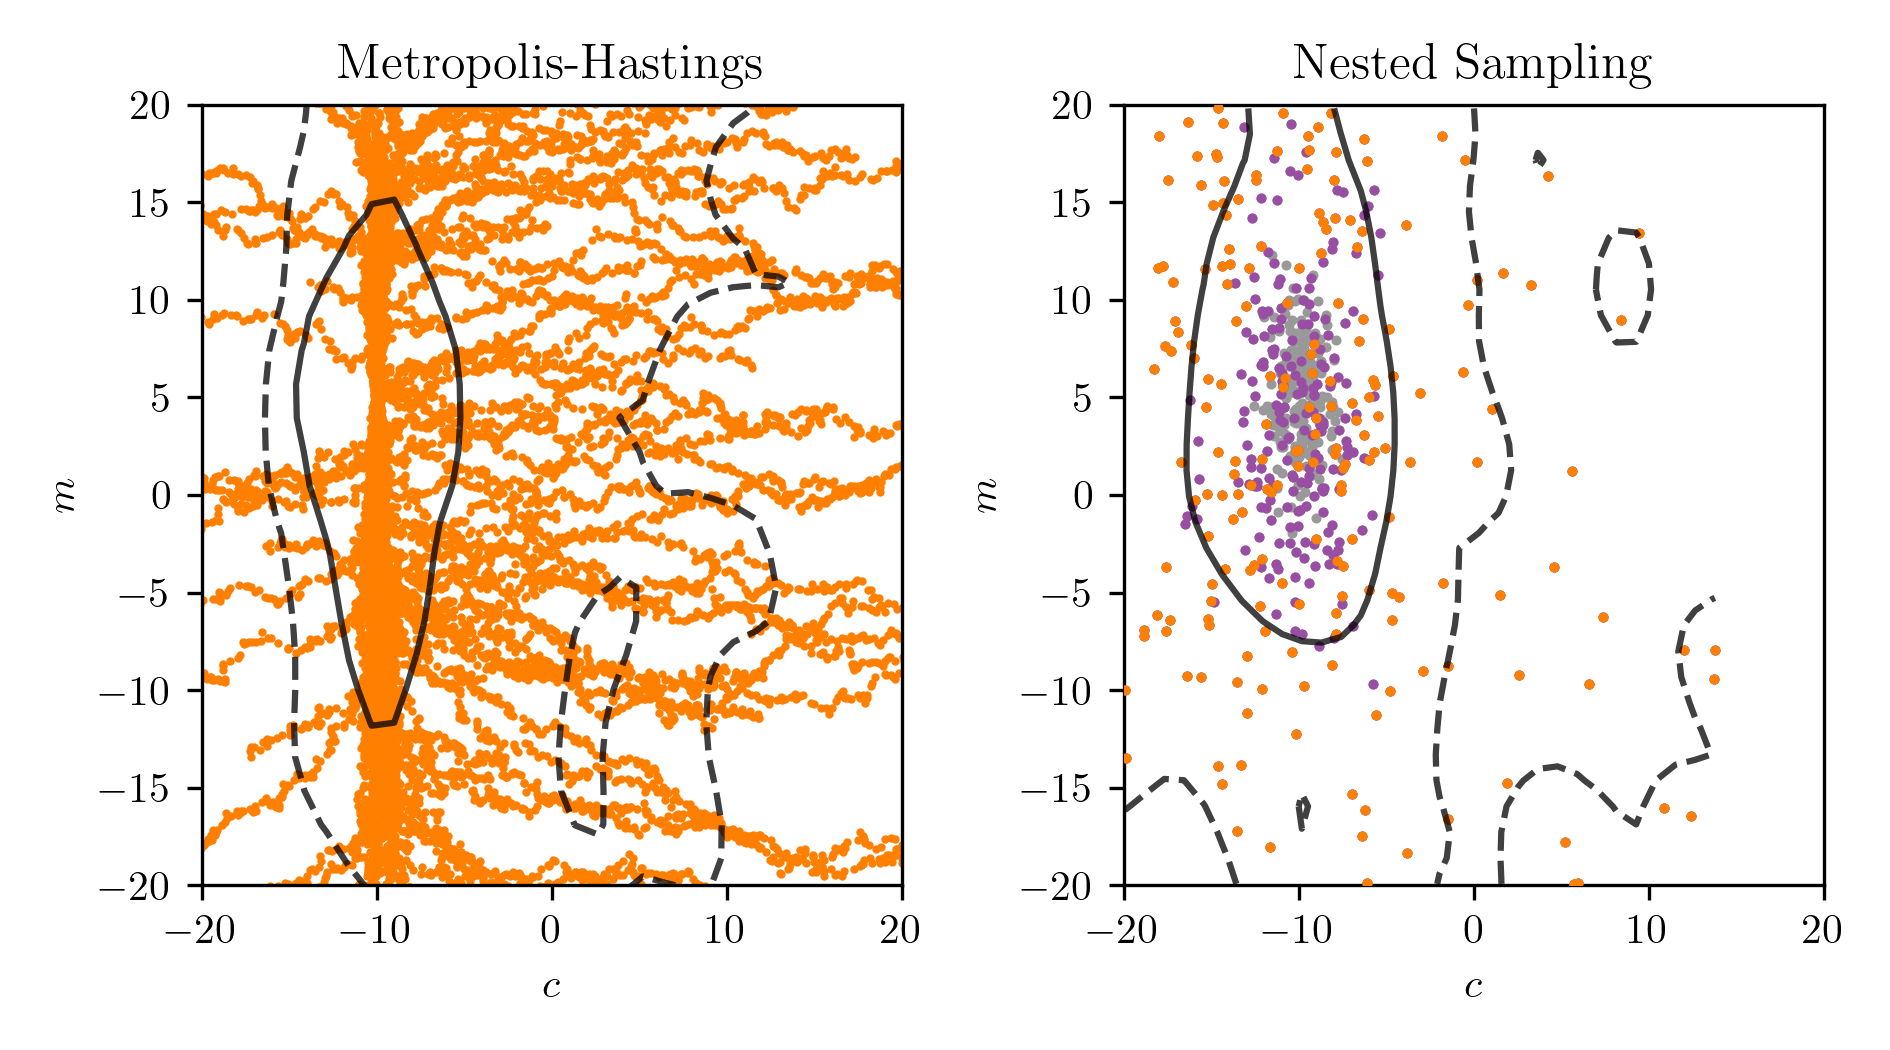
\includegraphics{introduction/figs/sampling_comparison.png}
    \caption{The figure shows a comparison of the random walk Metropolis-Hastings~(MH) sampling algorithm on the left and a rejection based Nested Sampling~(NS) algorithm on the right. The MH algorithm evolves 100 walkers for 250 steps each to explore the parameter space and the NS algorithm evolves 100 live points for 600 iterations. For more details see the text.}
    \label{fig:sampling_comparison}
\end{figure}

Bayesian inference is often performed with Markov Chain Monte Carlo~(MCMC) methods like the Metropolis-Hastings algorithm \cite{Hastings_MCMC_1970} and affine invariant ensemble samplers \cite{Foreman_Mackey_2013}. These approaches often produce unnormalised samples of the posterior and do not directly provide an estimate of the evidence.

A simple example of an MCMC sampler is the Metropolis-Hastings algorithm. In the left panel of \cref{fig:sampling_comparison} we show the resultant posterior found when fitting the gradient, $m$, and intercept, $c$, of a straight line given by
\begin{equation}
    y = mx + c + \epsilon,
\end{equation}
where $m = 5$ and $c=-10$ and the noise $\epsilon \sim \mathcal{N}(0, \sigma)$ is Gaussian distributed with a standard deviation of $\sigma = 0.5$.

The Metropolis-Hastings algorithm is a random walker algorithm that starts in some randomly chosen or carefully curated place, $x_0 = \{m_0, c_0\}$, often within some bounds, and subsequently gets perturbed in random directions. The direction of the perturbation is chosen based on some proposal distribution, which is equivalent to the prior. Here the proposal distribution of the next step, $x_{i+1}$, is given by a Gaussian centred around the previous step, $x_{i}$
\begin{equation}
    \pi(x_{i+1}|x_{i}) = \frac{1}{\sigma \sqrt{2\pi}}\exp\bigg(-\frac{1}{2}\frac{(x_{i+1} - x_{i})^2}{\sigma^2}\bigg),
\end{equation}
where we have set the standard deviation, $\sigma = 0.2$. At each iteration, the likelihood for the new point, $x_{i+1}$, is calculated, for example with \cref{eq:log_likelihood}, and compared to the equivalent value for $x_{i}$. The proposal or prior weighted ratio of the two likelihoods is taken
\begin{equation}
    \alpha = \frac{\mathcal{L}(x_{i+1}) \pi(x_{i+1})}{\mathcal{L}(x_{i})\pi(x_{i})},
\end{equation}
and compared to a random number, $u$, from a uniform distribution between $0 - 1$. If $u \leq \alpha$ then the new point is accepted into the chain else $x_{i}$ is perturbed again in a different random direction and the process is repeated. It is often more convenient to work in log-space because the likelihoods are very small, meaning that our inequality is given by
\begin{equation}
    \log_{10}(u) \leq \log_{10}(\alpha) = \log_{10}(\mathcal{L}(x_{i+1})) - \log_{10}(\mathcal{L}(x_{i})) + \log_{10}(\pi(x_{i+1})) - \log_{10}(\pi(x_{i})).
\end{equation}

The idea here is to climb up the likelihood contour but allow for occasional steps down the contours in an effort to prevent missing maxima in multi-modal problems. For example, in the case where the likelihood of step $x_{i+1}$ is higher than for step $x_{i}$ then $\alpha$ is always greater than 1 and always greater than $u$. However, if the likelihood for step $x_{i+1}$ is less than for $x_{i}$ then $\alpha < 1$ but if $u$ is randomly chosen to be less than $\alpha$ the step is accepted. This leads to a more complete exploration of the parameter space whilst maintaining a degree of efficiency and a focus on the maximum likelihood value. Through this process, the algorithm generates samples on the posterior distribution.

Here, the choice of $\sigma$ in the proposal distribution has a significant impact on how the algorithm converges. In fact, the functional form of the proposal distribution strongly impacts how the space is explored and the efficiency with which the maximum likelihood value is found. The samples from HERA used in \cref{ch:hera_saras3} were derived using ensemble MCMC techniques, where the new sample points are chosen based on the distribution of all the current live points or walkers \cite{Foreman_Mackey_2013, Ashton_ns_review_2022}.

In contrast, the Nested Sampling algorithm, used throughout this thesis, evolves a series of live points, $n_{\mathrm{live}}$, up the likelihood contour \cite{skilling_nested_2004, Ashton_ns_review_2022} in an effort to approximate the Bayesian evidence. The algorithm begins by evaluating the likelihood for the initial $n_{\mathrm{live}}$ points chosen from the prior distribution $\pi(\theta)$. The lowest likelihood point is then discarded and a new point is drawn from the prior with a higher likelihood than the discarded point. At each iteration the volume contained by the live points is compressed exponentially from an initial value of $X_0 = 1$, i.e. the prior, to $X_{i+1} = \exp(-1/n_\mathrm{live}) X_{i}$.% and the evidence is incremented by the product of the likelihood and $\Delta X / 2$. 

The evidence is therefore given by
\begin{equation}
    \mathcal{Z} = \sum^{n_\mathrm{iter}}_{i=1} w_i L^*_i
\end{equation}
where $L^*_i$ is the discarded likelihood at each iteration between $i=1$ and the total number of iterations $n_\mathrm{iter}$. The weights $w_i$ are given by
\begin{equation}
    w_i = \frac{1}{2}(X_{i+1} - X_{i-1}).
\end{equation}

The rejected sample at each iteration $i$ has an associated likelihood, weight, evidence and prior probability, which means that the Nested Sampling algorithm generates normalised samples on the posterior. We can then interpret this to tell us which parameter values in our prior ranges best describe the data.

Nested sampling is compared with the Metropolis Hastings algorithm in \cref{fig:sampling_comparison} using the same two-dimensional line fitting problem discussed previously.

The simplest sampling algorithm where a new sample is randomly drawn from the prior to replace the discarded point is slow, and alternatives such as slice sampling are much more efficient \cite{Neal_sampling_2000}. Slice sampling was originally implemented in a Nested Sampling algorithm in \cite{Aitken_sampling_2013} and extended in \cite{Handley2015a, Handley2015b} to work in higher dimensions. 

%In slice sampling we reject the lowest likelihood point, randomly select a point from the remaining live points and define a randomly chosen principle axis through that point. We then sample uniformly along a given length of that principle axis and if the likelihood of the new point is less than that of the rejected point we shrink the range along the axis that we are drawing samples from. The initial width of the slice is defined by the width of the likelihood contour, and the shrinking is designed to deal with multi-modal distributions. If the likelihood is larger, we pick another direction and repeat the process for a given number of repeats. We repeat the sampling to prevent the new point and the original point that we sliced through being correlated, and to be confident that the new point has been drawn from the prior.

Nested sampling algorithms typically rely on stopping criteria that determine the number of iterations to perform. It can become increasingly less rewarding to try to find replacement live points with higher likelihoods as you travel up the likelihood contours. A commonly used stopping criteria is when the fractional increase in the evidence is below some user specified tolerance
\begin{equation}
    \Delta \mathcal{Z}/Z < \mathrm{tol}.
\end{equation}

Bayesian inference techniques are well established in the field of cosmology and have been used for a number of years due to pioneering work analysing the CMB data~\cite{Trotta_bayes_2008}. However, it is only in the last few years, due to the increased interest in the field after the reported EDGES detection (see \cref{sec:current_results}), that Bayesian techniques have been applied to data from 21-cm cosmology experiments. 

For example, in an analysis of data from SARAS2 the authors used likelihood ratios, comparing fits with and without signal models, to rule out certain astrophysical scenarios for the global 21-cm signal \cite{Singh_saras2_2017}. The likelihood ratio is defined by
\begin{equation}
    \mathcal{R} = \frac{\mathcal{L}_{M, 1}}{\mathcal{L}_{M, 2}},
\end{equation}
and when its value is $> 1$ then model one is preferred over model two. While likelihood ratios give an intuitive means of determining whether one model is more probable relative to another, they are a \textit{relative} metric, unlike the Bayesian Evidence which is an absolute metric. Further, likelihood ratios do not appropriately account for the choice of prior, which the Bayesian Evidence does.

In an analysis of data from the EDGES high band instrument, the authors generated several million simulations of their data from a wide prior and calculated their corresponding likelihoods to estimate the posterior without using MCMC or Nested Sampling \cite{Monsalve_EDGES_HB_3_2019}. Finally, a significant number of experimental efforts have employed MCMC sampling to explore the astrophysical parameter space of the 21-cm power spectrum including LOFAR \cite{Ghara_LOFAR_2020} and MWA \cite{Ghara_MWA_2021}. 

Forward modelling of the global 21-cm signal in a Bayesian Nested Sampling pipeline has been pioneered by the REACH collaboration \cite{Anstey_REACH_2021, Anstey_antenna_2022}. Bayesian inference is employed significantly in this thesis, in which the Nested Sampling algorithm, implemented with \textsc{multinest} \cite{multinest_2008, multinest_2009, multinest_2019, PyMultiNest} and \textsc{polychord} \cite{Handley2015a, Handley2015b}, is used to model data from EDGES, LEDA, SARAS2, SARAS3, Planck, the Dark Energy Survey~(DES) and HERA.

\section{Machine learning and 21-cm Cosmology}
\label{sec:neural_networks}

Machine learning has many applications in the field of 21-cm cosmology. It has been shown that neural networks can capture the complex relationship between the 21-cm signal and the astrophysical process in the first billion years of cosmic history to a high degree of accuracy by \cite{Cohen2020} and more recently using two different approaches in \cite{Bevins_globalemu_2021} (\cref{ch:globalemu}) and \cite{21cmVAE}. The semi-numerical simulations that are used to model this signal take of order a few hours to produce per signal, whereas neural network emulators can produce estimates of these signals to varying degrees of accuracy in 10s of milliseconds. This is particularly important if we want to physically model signals in Bayesian Nested Sampling or MCMC runs where we are making thousands of calls to our signal generator, as in the latter half of this thesis.

In these scenarios, parameters, such as the star formation efficiency and virial circular velocity among others, are passed as inputs to a feed forward neural network and corresponding estimates of the 21-cm brightness temperature are output. An example network is shown in \cref{fig:neural_network}. In this example, the network takes two inputs, $p_1$ and $p_2$, and converts them to an output, $O_1$. Each node in the network is connected to all the nodes in the following layers, producing a `fully connected' feedforward network. When a numerical value is passed from one layer to the next, it is multiplied by the weight of the connection, $w_{ij}$ and a bias, $\beta_{ij}$ is added where $i$ corresponds to the node in the previous layer and $j$ the node in the next layer. For example, when $p_1$ is passed to the first node in the first layer, the value received is $w_{11} p_1 + \beta_{11}$. In addition, the node receives a weighted and shifted version of input $p_2$, since the network is fully connected, meaning that the value at node one (subscript) in layer one (superscript) is
\begin{equation}
    a_1^1 = w_{11} p_1 + w_{21} p_2 + \beta^1_1,
\end{equation}
where we define the bias at node one in layer one to be $\beta_1^1 = \beta_{11} + \beta_{21}$ or more generally $\beta_j^n =\sum_i \beta_{ij}$. The value at node one in layer one is scaled via an activation function into $a^{1 \prime}_1$. 

Activation functions can take many different forms and two examples, the sigmoid and linear, are shown in \cref{fig:neural_network}. The activation function is usually designed to introduce non-linearity in the network and allows the network to learn more complex relationships between the input and output. For this reason, the use of a linear output is often restricted to the final node and the sigmoid function is a common choice for the hidden layers, those between the input and output. $a^{1 \prime}_1$ is given by
\begin{equation}
    a^{1 \prime}_1 = \frac{1}{1+\exp(-a_{1}^1)}.
\end{equation}
$a^{1 \prime}_1$ is then passed to each node in the second layer and the process is repeated.

The number of layers and number of nodes in each layer is a choice for the user but can often be motivated by the demands of the problem as shown in \cref{ch:globalemu}. More complex structures in theory can model more complex relationships between the inputs and outputs of the network. However, arbitrarily increasing the size of the network can reduce the ability of the network to generalise to problems it has not seen before. This is a problem known as overfitting and is discussed in \cref{ch:globalemu} and \cite{Bevins_globalemu_2021}.

\begin{figure}[h!]
    \centering
    \begin{tikzpicture}[rednode/.style={circle, draw=red!60, fill=red!5, very thick, minimum size=5mm},
                bluenode/.style={circle, draw=blue!60, fill=blue!5, very thick, minimum size=5mm},
                greennode/.style={circle, draw=green!60, fill=green!5, very thick, minimum size=5mm},
                node distance=0.5cm and 2cm,
                remember picture]
        \node (0) {};
        \node[bluenode, above left=of 0, text width=0.5cm, align=center](input_1) {$p_1$};
        \node[bluenode, below left=of 0, text width=0.5cm, align=center](input_2) {$p_2$};

        \node[rednode, below right=of input_1, text width=0.5cm, align=center](layer1_center) {};
        \node[rednode, above=of layer1_center, text width=0.5cm, align=center](layer1_top) {};
        \node[rednode, below=of layer1_center, text width=0.5cm, align=center](layer1_bottom) {};

        \node[below=of layer1_bottom, inner sep=0pt] (sigmoid1) {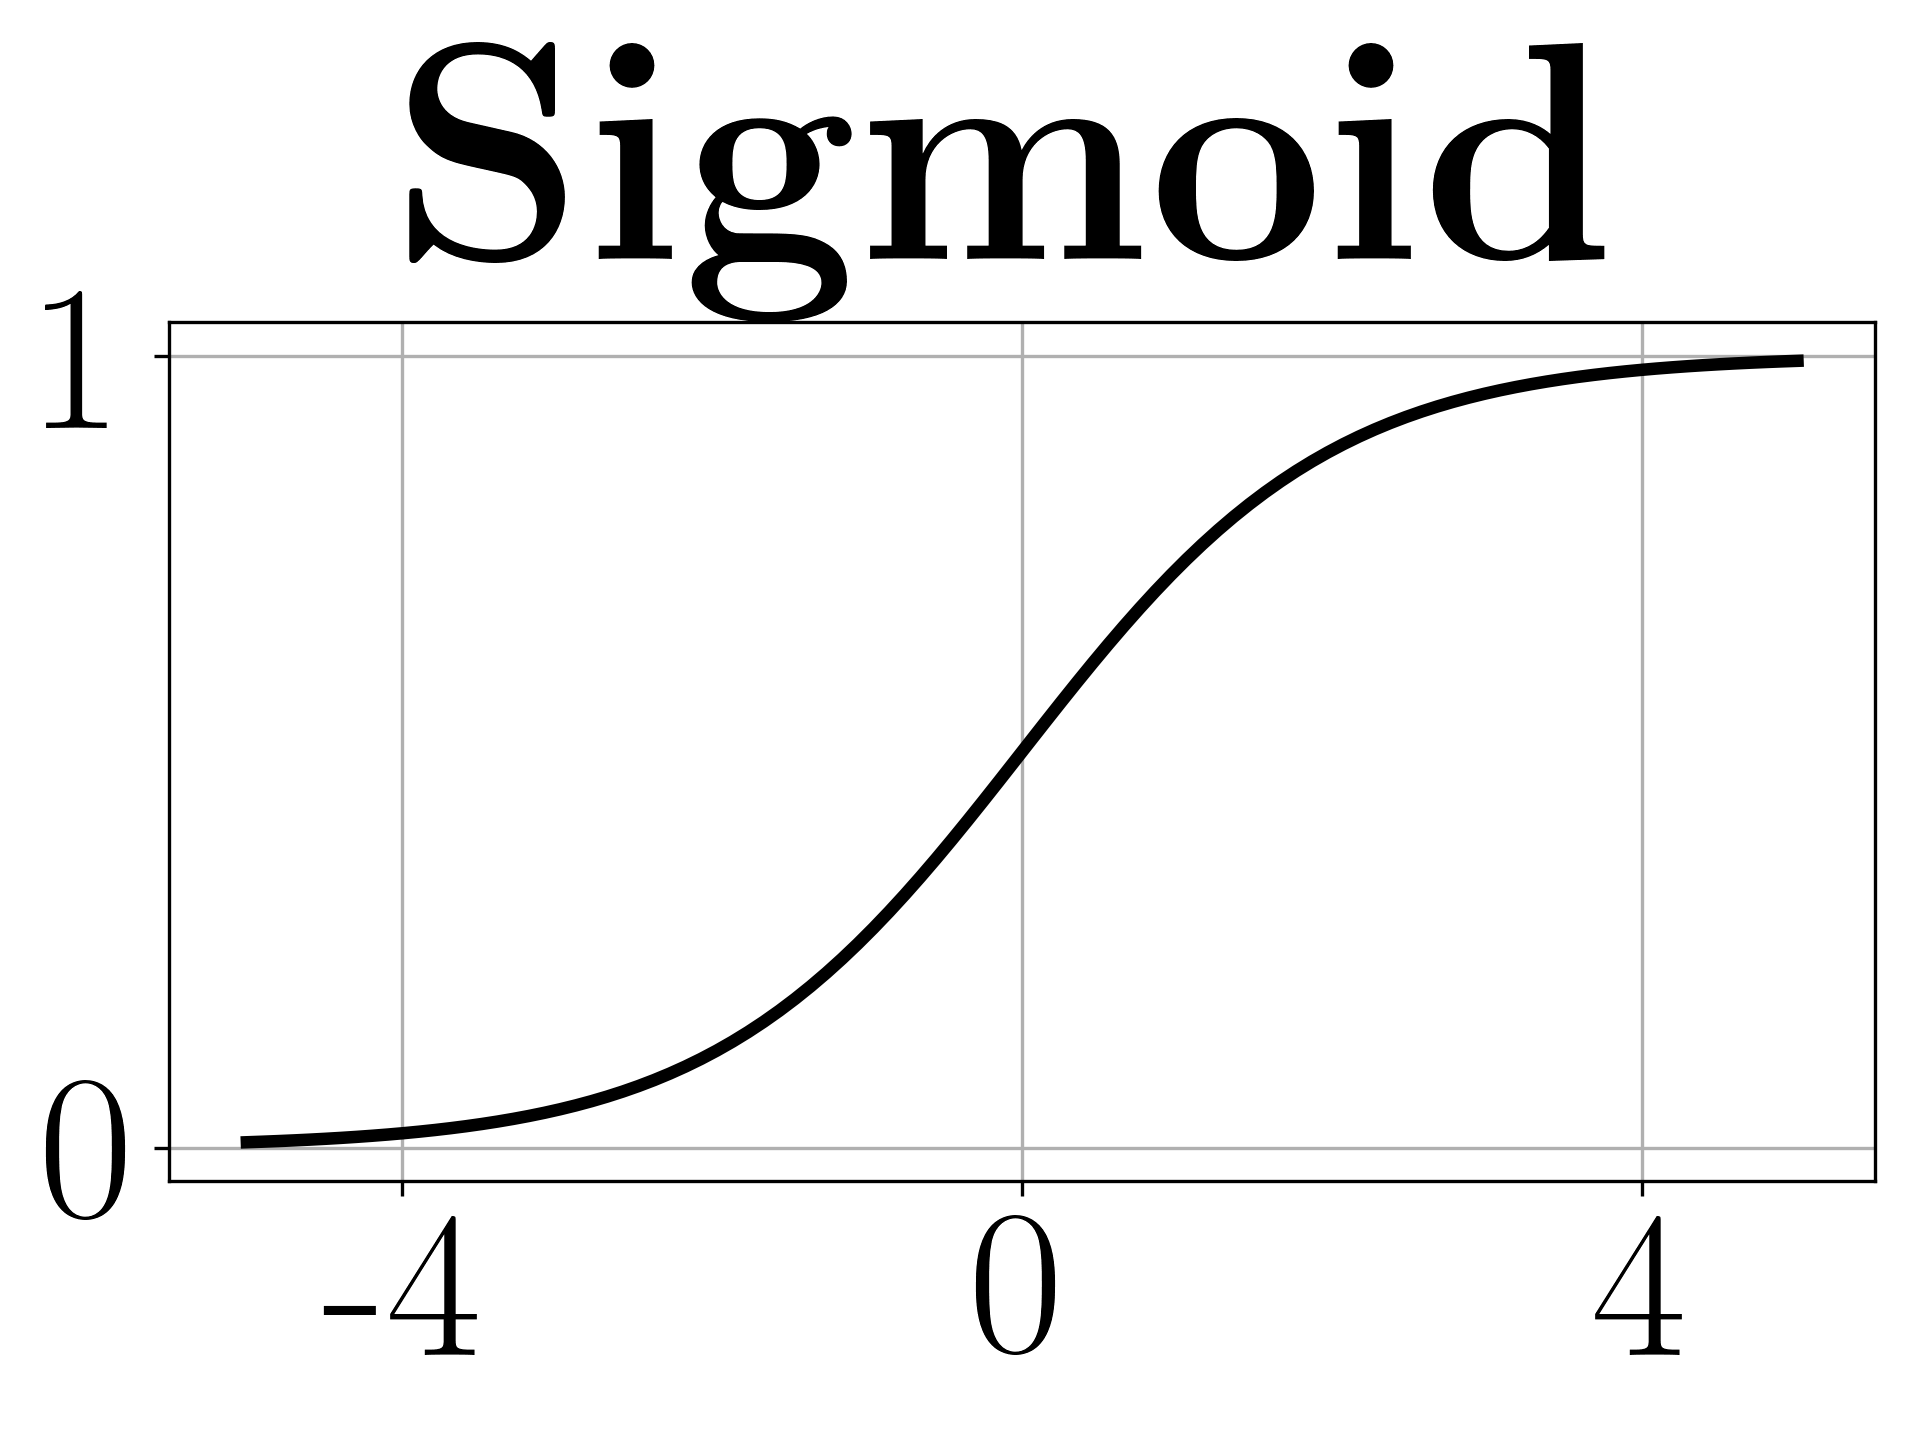
\includegraphics[width=.1\textwidth]{introduction/figs/sigmoid_function.png}};

        \node[rednode, right=of layer1_center, text width=0.5cm, align=center](layer2_center) {};
        \node[rednode, above=of layer2_center, text width=0.5cm, align=center](layer2_top) {};
        \node[rednode, below=of layer2_center, text width=0.5cm, align=center](layer2_bottom) {};

        \node[below=of layer2_bottom, inner sep=0pt] (sigmoid1) {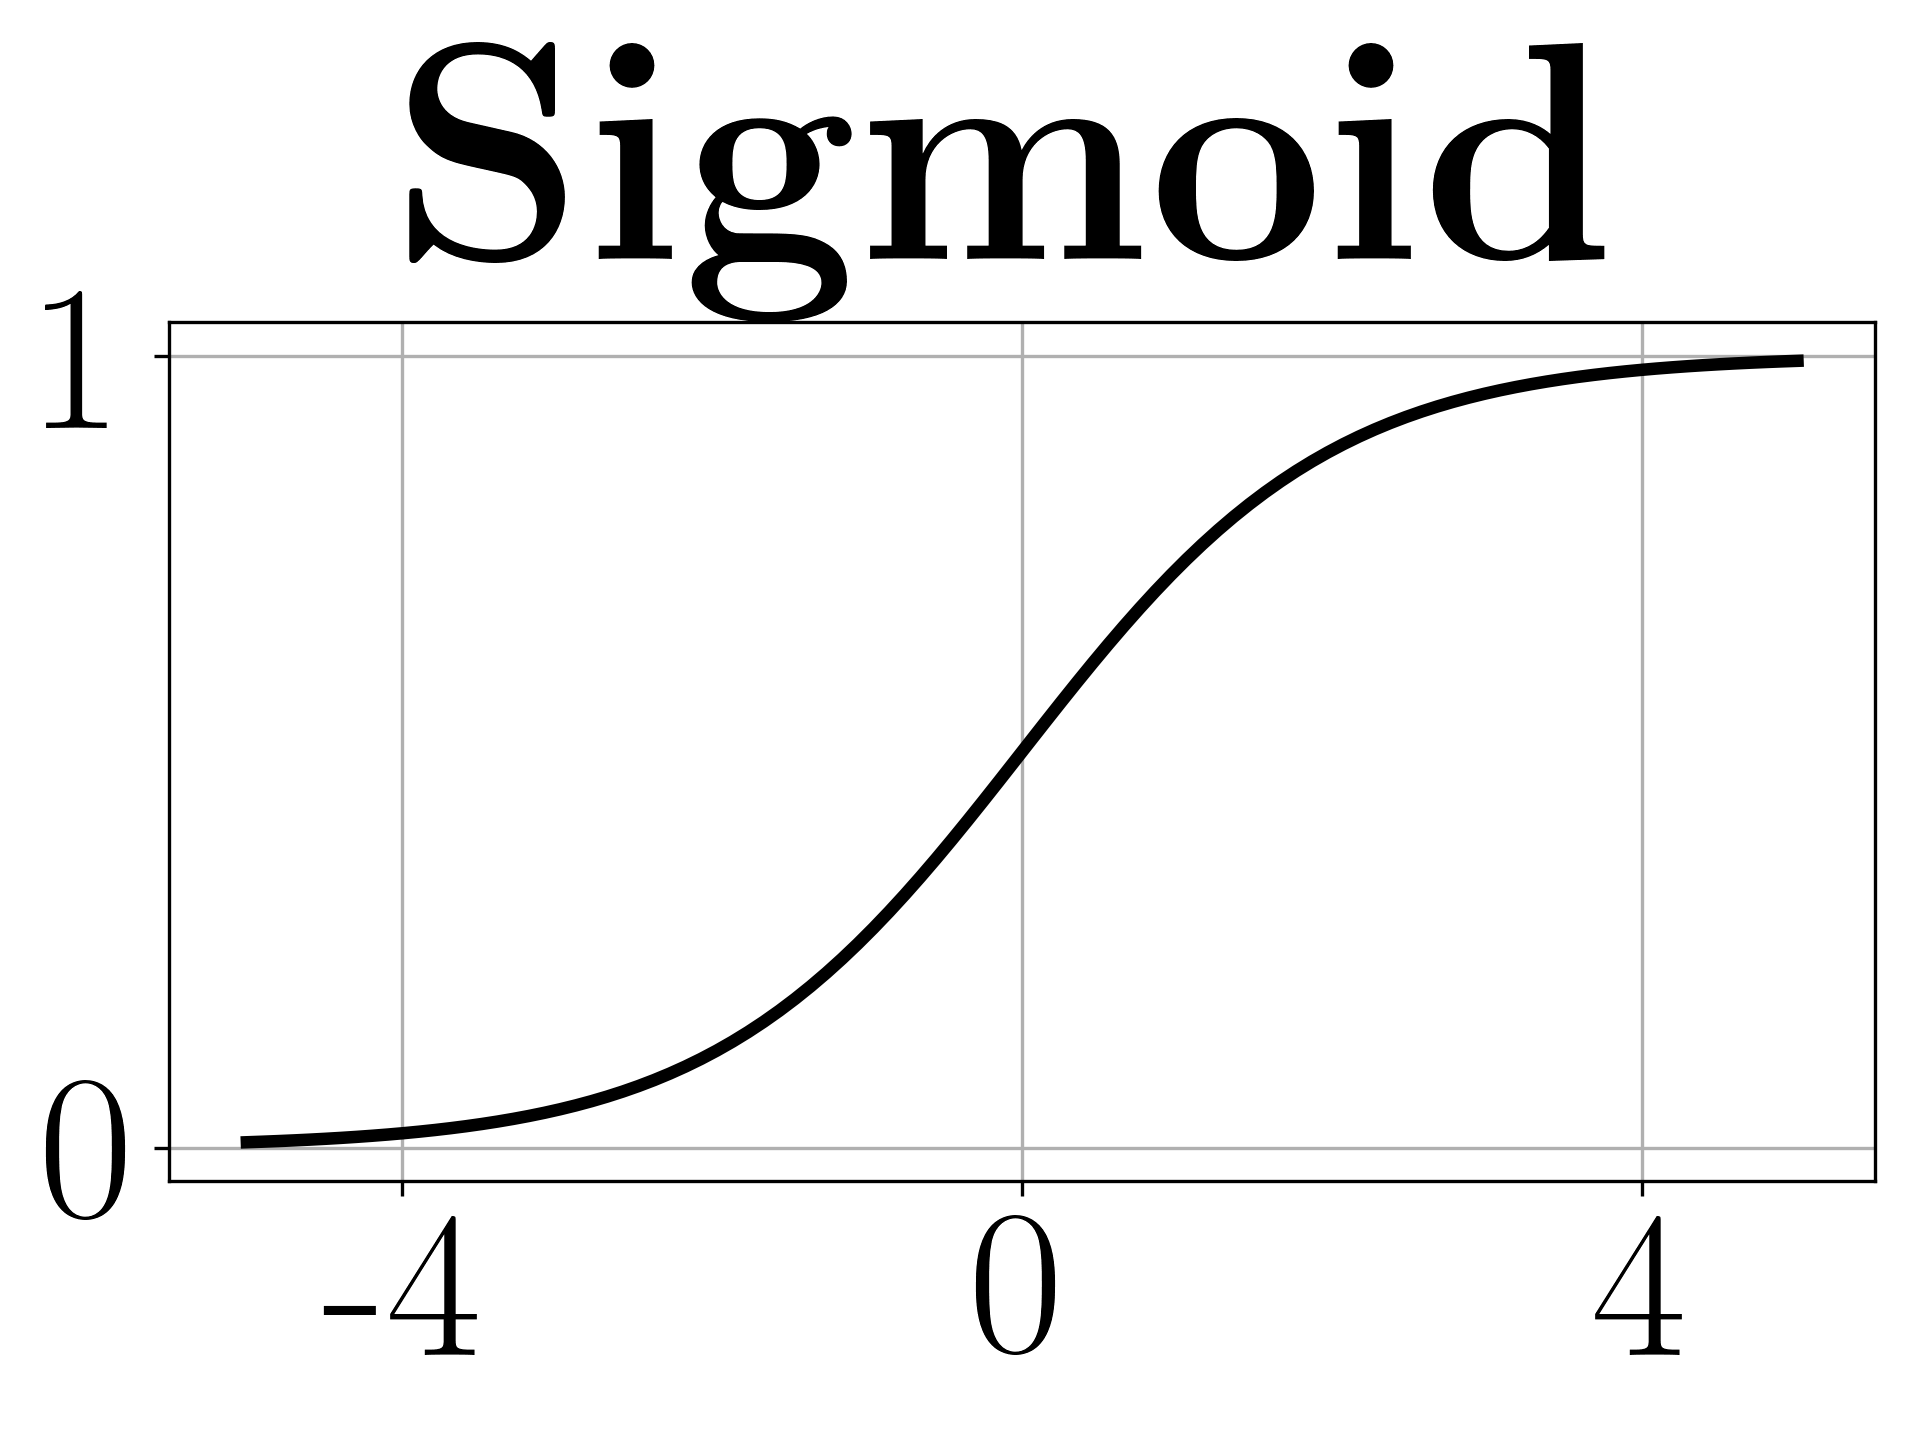
\includegraphics[width=.1\textwidth]{introduction/figs/sigmoid_function.png}};

        \node[greennode, right=of layer2_center, text width=0.5cm, align=center](output_1) {$O_1$};
        %\node[greennode, below right=of layer2_center, text width=0.5cm, align=center](output_2) {$O_2$};

        \node[below=of output_1, inner sep=0pt] (sigmoid1) {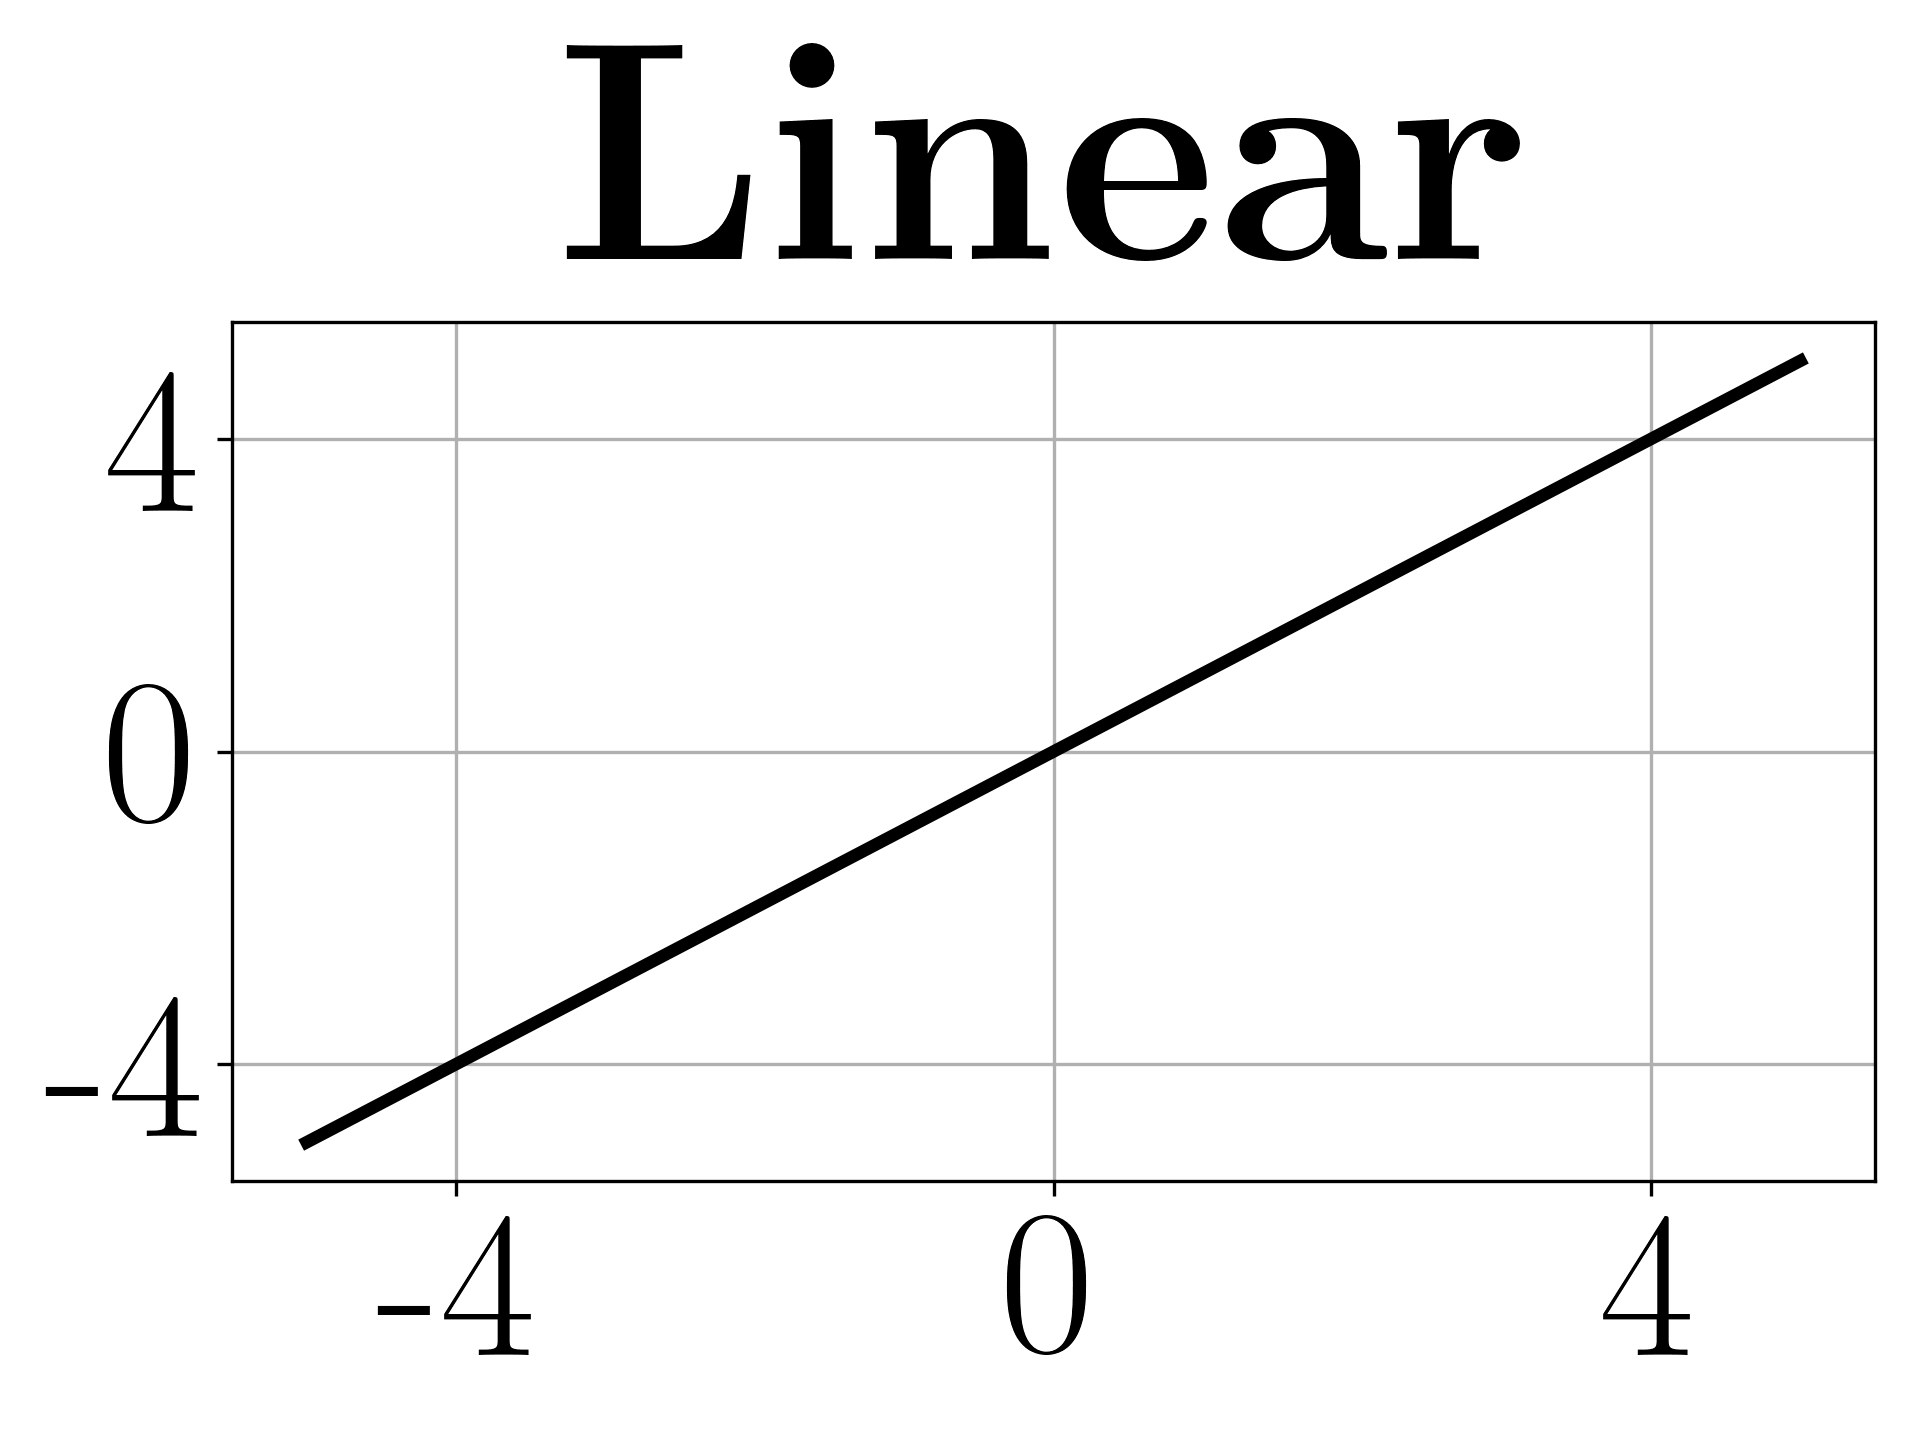
\includegraphics[width=.1\textwidth]{introduction/figs/linear_function.png}};

        \draw[->](input_1.east) -- (layer1_top.west) node[midway,above] {$w_{ij},~\beta_{ij}$};
        \draw[->](input_1.east) -- (layer1_bottom.west);
        \draw[->](input_1.east) -- (layer1_center.west);

        \draw[->](input_2.east) -- (layer1_top.west);
        \draw[->](input_2.east) -- (layer1_bottom.west);
        \draw[->](input_2.east) -- (layer1_center.west);

        \draw[->](layer1_bottom.east) -- (layer2_top.west);
        \draw[->](layer1_bottom.east) -- (layer2_center.west);
        \draw[->](layer1_bottom.east) -- (layer2_bottom.west);

        \draw[->](layer1_center.east) -- (layer2_top.west);
        \draw[->](layer1_center.east) -- (layer2_center.west);
        \draw[->](layer1_center.east) -- (layer2_bottom.west);

        \draw[->](layer1_top.east) -- (layer2_top.west) node[midway,above] {$w_{ij},~\beta_{ij}$};
        \draw[->](layer1_top.east) -- (layer2_center.west);
        \draw[->](layer1_top.east) -- (layer2_bottom.west);

        \draw[->](layer2_bottom.east) -- (output_1.west);

        \draw[->](layer2_center.east) -- (output_1.west);

        \draw[->](layer2_top.east) -- (output_1.west) node[midway,above right] {$w_{ij},~\beta_{ij}$};
    \end{tikzpicture}
    \caption{The diagram shows a simple feed forward neural network that takes two input parameters, $p_1$ and $p_2$, and transforms that to an output, $O_1$. $w_{ij}$ and $\beta_{ij}$ represent the weights and biases between layer $i$ and layer $j$. The diagrams at the bottom of the figure show two different activation functions which in the hidden layers of the network, those between the input and output, are designed to introduce non-linear structure into the model.}
    \label{fig:neural_network}
\end{figure}

The issue is therefore how to set the weights and biases of the neural network. These have to be learned based on some training data that we give to the network, i.e. a set of inputs and corresponding outputs, and a loss function. The loss function is chosen by the user, but typically we use a root mean squared error (or RMSE) loss given by
\begin{equation}
    \sigma_{NN} = \sqrt{\frac{1}{N}\sum (y_\mathrm{true}-y_\mathrm{pred})^2},
    \label{eq:loss_intro}
\end{equation}
where $y_\mathrm{true}$ is the true value of the output and $y_\mathrm{pred}$ is what the network predicts.

In \cref{eq:loss_intro}, $y_\mathrm{pred}$ is a function of the weights and biases of the network, and therefore we can say the same of the loss function, $\sigma_{NN}(\mathbf{w}, \mathbf{\beta})$. In order to optimize the values of the weights and biases, we minimise the loss function using a gradient descent algorithm, where at iteration $i+1$ the weights are updated according to
\begin{equation}
    \mathbf{w}_{i+1} = \mathbf{w}_i - \gamma \nabla \sigma(\mathbf{w}_i, \mathbf{\beta}_i),
\end{equation}
where $\gamma$ is known as the learning rate and determines the size of the step taken in the parameter space. The gradient effectively tells us which connections in the network have the largest impact on the loss. To evaluate the negative gradient of the loss function with respect to the weights and biases, we use the backpropagation algorithm.

The backpropagation algorithm begins by looking at how the weights and biases between the output and the previous layer need to change to improve the loss function for a particular example. To calculate the gradient of the loss with respect to each weight and bias between the output and the previous layer in the above example, we rely on the chain rule
\begin{equation}
    \frac{\delta \sigma}{\delta w^2_{ij}} = \frac{\delta \sigma}{\delta O_1} \frac{\delta O_1}{d w^2_{ij}}.
\end{equation}
For intermediate layers between the output and input there is an additional term accounting for the impact of the activation function. Since the output activation, the loss and the hidden layer nodes are known functions, we can use Automatic Differentiation to calculate their derivatives with respect to each weight and bias. Once we have expressions for all the derivatives, the algorithm updates the weights according to
\begin{equation}
    w^2_{ij} - \gamma \frac{\delta \sigma}{\delta w^2_{ij}}.
\end{equation}
starting with the weights between the input and the first hidden layer and propagating the change forward.
%The process, then propagates back through the network using the modified weights and biases between the output and the previous layer until all the weights and biases have been adjusted appropriately.
The algorithm calculates the required changes in the weights and biases for a series of training examples, and then averages the changes over many examples to try to improve the accuracy of the network while maintaining the ability for it to generalise to unseen test examples. 

We could do this for all examples in our training data and perform a gradient descent. However, this is a very computationally expensive task. For example, the network shown in \cref{fig:neural_network} has 18 weights and biases creating a 36 dimensional space to optimize and consequently training neural networks is non-trivial and there are many tricks that can be employed to try and improve their accuracy. Some of these are discussed in \cref{ch:globalemu}. However, the most basic trick typically employed is to divide the training data into batches and perform a stochastic gradient descent. The algorithm picks the most appropriate direction to move each weight and bias, and determines by how much to move them to improve the loss function for a specific subset of randomly chosen training examples. Doing this over many iterations for many batches, while sometimes increasing the loss for the whole training data set, eventually finds a good approximation to the true minimum or a local minimum that sufficiently optimizes the network and is much more computationally efficient than a full gradient descent. %The algorithm effectively up weights the most important inputs, or features, with respect to the output while allowing it to perform well on unseen data.

The neural network emulator \textsc{globalemu} discussed in \cref{ch:globalemu} is a typically small feed forward network. The previous state of the art global 21-cm signal emulator \textsc{21cmGEM} relies on several such networks and a decision tree \cite{Cohen2020}. The recently published \textsc{21cmVAE} relies on a Variational Autoencoder to compress the input parameter space into a lower dimensional latent space in which to learn the relationship with the output 21-cm signal \cite{21cmVAE}.  \textsc{globalemu} and \textsc{21cmVAE} represent the `next generation' emulators and the latter is more accurate but around 40 times slower than \textsc{globalemu}. Both emulators and \textsc{21cmGEM} are sufficiently accurate for the current noise levels in present experimental efforts. Recently, some of the techniques used in the development of \textsc{globalemu} have been applied to the emulation of the 21-cm power spectrum in the HERA analysis \cite{HERA_2022c}. %In global 21-cm cosmology the inverse problem, where the raw data is input and astrophysical parameters are output, is also possible and has been previously attempted \cite{Choudhury_2021}.

In \cref{ch:margarine}, we discuss a different type of machine learning algorithm known as a Masked Autoregressive Flow~(MAFs). MAFs are a form of normalising flow that string together a series of Masked Autoencoder for Distribution Estimation~(MADE) \cite{Germain_MADE_2015} networks to perform density estimation. They are an example of a Neural Density Estimator. Normalising flows allow us to calculate the log-probability, $\log(P(x))$, for a set of samples $\{x\}$ on some complex distribution. We assume that the multidimensional distribution $P(x)$ can be decomposed into a set of one-dimensional conditional distributions
\begin{equation}
P(x) = \prod_i P(x_i| x_1, x_2, ..., x_{i-1}),
\end{equation}
where the index $i$ represents the dimension. We model each conditional probability as a Gaussian distribution and assume a base standard normal distribution, $\mathcal{N}(0, 1)$, that is shifted and scaled by some standard deviation, $\sigma_i$, and mean, $\mu_i$, which can be written as
\begin{equation}
P(x_i| x_1, x_2, ..., x_{i-1}) = \mathcal{N}(\mu_i(x_1, x_2, ..., x_{i-1}), \sigma_i(x_1, x_2, ..., x_{i-1})),
\end{equation}
or alternatively written in terms of samples in $x_i$
\begin{equation}
x_i = \sigma_i z_i + \mu_i,
\end{equation}
where $z_i \sim \mathcal{N}(0, 1)$. The problem is how to estimate the appropriate set of $\sigma_i$ and $\mu_i$ to model the distribution of $x_i$. We do this with the MADE architecture which is shown in \cref{fig:maf} (see also \cite{Alsing2019}) and the change of variables principle
\begin{equation}
    P(x) = P(z) \bigg|\frac{\delta z}{\delta x}\bigg|
\end{equation}
which describes how one probability distribution can be transformed into another. Here the magnitude of the determinant of the Jacobian represents the change in volume between $P(x)$ and $P(z)$ and it ensures that $P(x)$ is normalised hence `normalising' flows.

\begin{figure}[h!]
    \centering
    \begin{tikzpicture}[rednode/.style={circle, draw=red!60, fill=red!5, very thick, minimum size=5mm},
                bluenode/.style={circle, draw=blue!60, fill=blue!5, very thick, minimum size=5mm},
                greennode/.style={circle, draw=green!60, fill=green!5, very thick, minimum size=5mm},
                node distance=0.5cm and 2cm,
                remember picture]
        \node (0) {};
        
        \node[rednode, above=of 0, text width=0.5cm, align=center](layer1_center1) {$\mu_2$};
        \node[rednode, below=of layer1_center1, text width=0.5cm, align=center](layer1_center2) {$\sigma_2$};
        \node[rednode, above=of layer1_center1, text width=0.5cm, align=center](layer1_top2) {$\sigma_1$};
        \node[rednode, above=of layer1_top2, text width=0.5cm, align=center](layer1_top1) {$\mu_1$};
        \node[rednode, below=of layer1_center2, text width=0.5cm, align=center](layer1_bottom1) {$\mu_3$};
        \node[rednode, below=of layer1_bottom1, text width=0.5cm, align=center](layer1_bottom2) {$\sigma_3$};
    
        \node[rednode, left=of layer1_top2, text width=0.5cm, align=center](hl1) {};
        \node[rednode, left=of layer1_center1, text width=0.5cm, align=center](hl2) {};
        \node[rednode, left=of layer1_center2, text width=0.5cm, align=center](hl3) {};
        \node[rednode, left=of layer1_bottom1, text width=0.5cm, align=center](hl4) {};
        
        \node[below=of hl4, inner sep=0pt] (tanh) {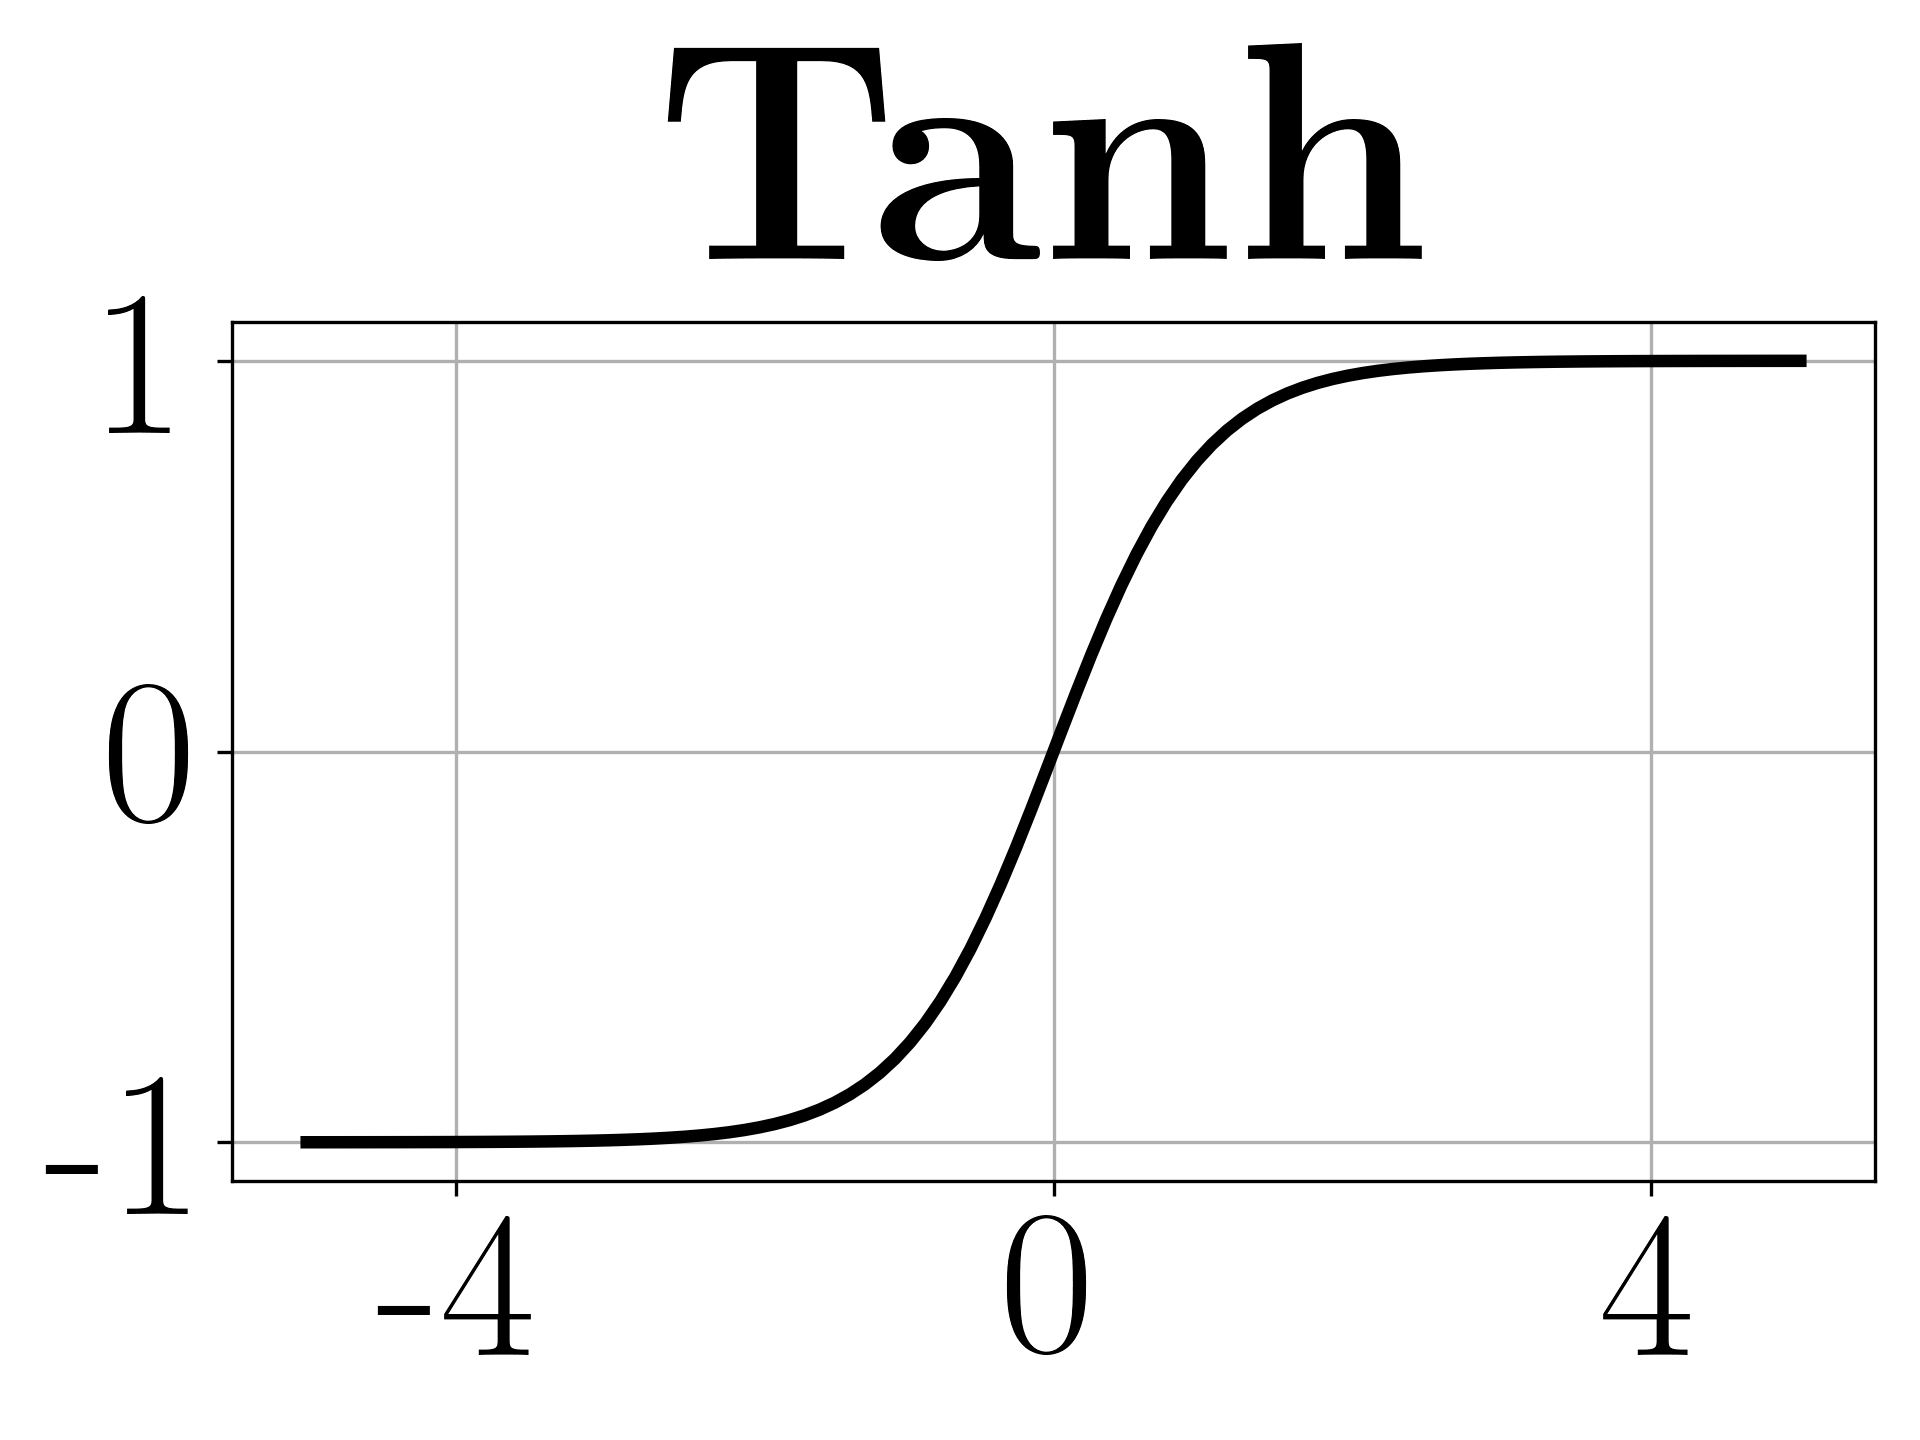
\includegraphics[width=.1\textwidth]{introduction/figs/tanh_function.png}};
        
        \node[bluenode, below left=of hl2, text width=0.5cm, align=center, yshift=0.3cm](input_2) {$x_2$};
        \node[bluenode, above=of input_2, text width=0.5cm, align=center, yshift=0.12cm](input_1) {$x_1$};
        \node[bluenode, below=of input_2, text width=0.5cm, align=center, yshift=0.1cm](input_3) {$x_3$};

        \node[greennode, right=of 0, text width=0.5cm, align=center, yshift=0.3cm](output_2) {$z^\prime_2$};
        \node[greennode, above=of output_2, text width=0.5cm, align=center, yshift=0.12cm](output_1) {$z^\prime_1$};
        \node[greennode, below=of output_2, text width=0.5cm, align=center, yshift=0.1cm](output_3) {$z^\prime_3$};
        
        \node[right=of output_2, align=left, xshift=-1.5cm, yshift=0.12cm] {$= (x_2 -\mu_2) / \sigma_2$};
        
        \node[right=of output_1, align=left, xshift=-1.5cm, yshift=0.12cm] {$= (x_1 -\mu_1) / \sigma_1$};
        
        \node[right=of output_3, align=left, xshift=-1.5cm, yshift=0.12cm] {$= (x_3 -\mu_3) / \sigma_3$};
        
        \draw[densely dashed](input_1.east) -- (output_1.west);
        
        \draw[densely dashed](input_2.east) -- (output_2.west);
        
        \draw[densely dashed](input_3.east) -- (output_3.west);
        
        \draw[->](input_1.east) -- (hl1.west);
        \draw[->](input_1.east) -- (hl2.west);
        \draw[->](input_1.east) -- (hl3.west);
        \draw[->](input_1.east) -- (hl4.west);
        
        %\draw[->](input_2.east) -- (hl1.west);
        %\draw[->](input_2.east) -- (hl2.west);
        \draw[->](input_2.east) -- (hl3.west);
        \draw[->](input_2.east) -- (hl4.west);
        
        %\draw[->](input_3.east) -- (hl1.west);
        %\draw[->](input_3.east) -- (hl2.west);
        %\draw[->](input_3.east) -- (hl3.west);
        %\draw[->](input_3.east) -- (hl4.west);
        
        \draw[->](hl1.east) -- (layer1_center1.west);
        \draw[->](hl2.east) -- (layer1_center1.west);
        %\draw[->](hl3.east) -- (layer1_center1.west);
        %\draw[->](hl4.east) -- (layer1_center1.west);
        
        \draw[->](hl1.east) -- (layer1_center2.west);
        \draw[->](hl2.east) -- (layer1_center2.west);
        %\draw[->](hl3.east) -- (layer1_center2.west);
        %\draw[->](hl4.east) -- (layer1_center2.west);
        
        %\draw[->](hl1.east) -- (layer1_top1.west);
        %\draw[->](hl2.east) -- (layer1_top1.west);
        %\draw[->](hl3.east) -- (layer1_top1.west);
        %\draw[->](hl4.east) -- (layer1_top1.west);
        
        %\draw[->](hl1.east) -- (layer1_top2.west);
        %\draw[->](hl2.east) -- (layer1_top2.west);
        %\draw[->](hl3.east) -- (layer1_top2.west);
        %\draw[->](hl4.east) -- (layer1_top2.west);
        
        \draw[->](hl1.east) -- (layer1_bottom2.west);
        \draw[->](hl2.east) -- (layer1_bottom2.west);
        \draw[->](hl3.east) -- (layer1_bottom2.west);
        \draw[->](hl4.east) -- (layer1_bottom2.west);
        
        \draw[->](hl1.east) -- (layer1_bottom1.west);
        \draw[->](hl2.east) -- (layer1_bottom1.west);
        \draw[->](hl3.east) -- (layer1_bottom1.west);
        \draw[->](hl4.east) -- (layer1_bottom1.west);
        
        \draw[densely dashed](layer1_top1.east) -- (output_1.west);
        \draw[densely dashed](layer1_top2.east) -- (output_1.west);
        
        \draw[densely dashed](layer1_center1.east) -- (output_2.west);
        \draw[densely dashed](layer1_center2.east) -- (output_2.west);
        
        \draw[densely dashed](layer1_bottom1.east) -- (output_3.west);
        \draw[densely dashed](layer1_bottom2.east) -- (output_3.west);

    \end{tikzpicture}
    \caption{The MADE architecture, when trained appropriately, transforms samples from a complex probability distribution $\{x\}$ on to samples from a standard normal distribution under the assumption that the probability distribution $\{x\}$ can be broken into conditional one-dimensional probability distributions represented as Gaussians. Many different MADE networks can be stacked together and trained to produce a normalising flow increasing the expressivity of the density estimation. By definition normalising flows are bijective, and a trained implementation can be used to calculate $\log(P(x))$ and draw samples from $P(x)$.}
    \label{fig:maf}
\end{figure}

The MADE architecture takes in sets of samples from $\{x\}$ and estimates the value of $\mu_i$ and $\sigma_i$ needed to transform them to samples on the standard normal distribution $\{z\}$. Doing this for many sets of samples in $\{x\}$ adjusts the networks weights and biases appropriately to transform the distribution as a whole. The base of the MADE architecture is a fully connected neural network like that in \cref{fig:neural_network} however certain connections are masked out to represent the fact that probability distributions and hence $\mu_i$ and $\sigma_i$ are conditional on samples from $x_{i-1}$ dimensions. The masking is performed by multiplying the matrices of associated weights with a binary mask.

$\sigma_i$ and $\mu_i$ are functions of the weights and biases in the MADE network, which can have multiple hidden layers with varying activation functions.%, and the idea is to minimise the loss function
%\begin{equation}
%    \mathrm{min}(\log(P(z^\prime)) + \log(\bigg|\frac{\delta z^\prime}{\delta x}\bigg|)),
%\end{equation}
%where here the change of variables is from the true standard normal distribution to the output of the neural network $z^\prime_i = (x_i - \mu_i)/\sigma_i$ which should, subject to appropriately chosen $\mu_i$ and $\sigma_i$, look identical. By minimising the above we are minimising the volume contraction between the output samples and the expected standard normal distribution thus generating an invertible transformation from the standard normal to  our target distribution $\{x\}$. 
The idea is to minimize the Kullback-Leibler~(KL) divergence between the true probability distribution of the samples $x$ and the prediction from the network $P_\theta(x)$ given by
\begin{equation}
    \mathcal{D} (P(x)||P_{\theta}(x)) = -\mathbb{E}_{P(x)}[\log P_\theta(x)] + \mathbb{E}_{P(x)}[\log P(x)],
\end{equation}
where $\theta$ represents the hyperparameters of the network. The second term in the KL divergence is independent of the network and so for a minimization problem we can ignore this and
\begin{equation}
    -\mathbb{E}_{P(x)}[\log P_\theta(x)] = -\frac{1}{N} \sum_{1=0}^N \log P_\theta(x_i),
\end{equation}
meaning that our minimization problem becomes
\begin{equation}
    \argmax_\theta \sum^N_{i=0} \log P_\theta(x_i),
\end{equation}
or equivalently by a change of variables
\begin{equation}
    \argmax_\theta \sum_{i=0}^N [\log P_\theta(z_i^\prime) + \log \bigg|\frac{\delta z_i^\prime}{\delta x_i}\bigg|],
\end{equation}
where $z^\prime$ is a function of $\theta$ \cite{Alsing2019}. Here the second term is just the derivative over the network and the first term is trivially calculated from the output $\sigma$ and $\mu$.

We can stack many such networks together and train them in unison to transform more complicated networks under the following
\begin{equation}
    \begin{split}
    \mathbf{z}_0 & = \mathcal{N}(0, 1) \\
    \mathbf{z}_1 & = \mathbf{z}_0 \boldsymbol{\sigma}_1(\mathbf{z}_0, \mathbf{w}) + \boldsymbol{\mu}_1(\mathbf{z}_0, \mathbf{w})\\
    \vdots &\\
    \mathbf{x} & = \mathbf{z}_{n-1} \boldsymbol{\sigma}_n(\mathbf{z}_{n-1}, \mathbf{w}) + \boldsymbol{\mu}_n(\mathbf{z}_{n-1}, \mathbf{w}),
    \end{split}
\label{eq:MAF}
\end{equation}
in a normalising flow. Here $\mu_j$ and $\sigma_j$ are $N$-dimensional vectors, $\mathbf{z}_0$ is our multidimensional standard normal distribution and $\mathbf{x}$ is the multidimensional target distribution. The intermittent $\mathbf{z}_j$ distributions are output from one MADE and passed to the next and the weights and biases are adjusted across the whole chain at each training step. The transformation performed by a normalising flow is bijective in that there is a one-to-one relationship between samples in the base distribution and the target distribution, so we can go back and forth between the two passing the emulator samples on the standard normal distribution and recovering samples on the input posterior for example. Normalising flows and MAFs have many applications which are discussed in \cref{ch:margarine}.

There are many additional applications of machine learning in the field of 21-cm cosmology such as the use of Convolutional Neural Networks to accurately emulate tomographic images of the 21-cm field and modelling foregrounds in power spectrum analysis. However, we refer the reader to the literature for more details as the focus of this thesis is primarily on the global 21-cm signal.

\section{Current experimental results}
\label{sec:current_results}

The 21-cm line from neutral hydrogen has long been understood to be a powerful probe of galactic physics \cite{Furlanetto_review_2006, Barkana_review_2016, Mesinger2019}. However, it is only in the past 20-30 years that its potential usefulness as a cosmological probe has really been explored (see the historical review in \cite{Furlanetto_review_2006}). Making tomographic images of the 21-cm signal as a function of redshift was first proposed in \cite{Madau1997} and is a target of the upcoming Square Kilometre Array~(SKA) \cite{Mellema_SKA_2013}.

To date, observational efforts have focused on two different but related statistics known as the 21-cm power spectrum and global or sky-averaged 21-cm signal. Detection of the 21-cm power spectrum has been attempted by a number of different telescopes including LOFAR \citep[LOw-Frequency ARray,][]{LOFAR_current_EoR_2018, Gehlot_lofar_2019, Ghara_LOFAR_2020, Mondal_LOFAR_2020, Greig_LOFAR_2021}, MWA \citep[Murchison Widefield Array,][]{Trott_mwa_2020, Greig_MWA_2020, Ghara_MWA_2021}, HERA \cite{HERA_2017, HERA_2022b} and GMRT \citep[Giant Metrewave Radio Telescope,][]{GMRT2011}. However, current observations are limited by our understanding of the systematics in the data.

The global 21-cm signal is in principle easier to detect than the power spectrum. Observations were first proposed in \cite{Shaver1999} and a number of ongoing experimental efforts are underway to detect this signal. While the detection of the power spectrum requires the use of an interferometer to measure the temperature variation across different angular scales on the sky, the global 21-cm signal can be detected, in principle, with a single antenna. A number of different experiments have attempted to make detections, are currently underway or have been proposed to make this measurement, including EDGES \cite{Bowman_edges_2018, EDGES_high_band_experimental_paper_2017}, SARAS \cite{SARAS2_radiometer_2018, SARAS_reciever_2021, SARAS3_antenna_2021, SARAS3_spectrometer_2020}, LEDA \cite{Price_LEDA_2018}, SCI-HI \citep[Sonda Cosmol\'{o}gica de las Islas para la Detecci\'{o}n de Hidr\'{o}geno Neutro,][]{SCIHI}, BIGHORNS \citep[Broadband Instrument for Global HydrOgen ReioNisation Signal,][]{BIGHORNS}, PRIZM \cite{Philip_PRIZM_2019}, MIST \citep[Mapper of the IGM Spin Temperature,][]{MIST}, FARSIDE \citep[Farside Array for Radio Science Investigations of the Dark ages and Exoplanets,][]{Burns_Moon_2021}, and REACH \cite{Acedo_REACH_2019, Anstey_REACH_2021,Cumner_antenna_2021, Anstey_antenna_2022, de_lera_acedo_reach_2022}.

In the following subsections, we explain the state of the field up to 2019, the start of this PhD, with some reference to more recent experimental results such as SARAS3 and HERA which are explored more in the main text. Part III of this thesis and the corresponding chapters detail improvements to our current understanding of the early Universe that I have been responsible for leading.

\subsection{The sky-averaged 21-cm signal}

A tentative detection of the global 21-cm signal was reported by the EDGES collaboration in 2018 \cite{Bowman_edges_2018}. If true, the detection implies rapid star formation, delayed and then rapid X-ray heating, an earlier than expected end to the epoch of reionization and exotic astrophysics such as an increased radio background \cite{FengRB2018, JanaRB2018, EwallRB2018, MirochaRB2019, Reis2020} or interactions between Baryons and Dark Matter \cite{MunozDM2018, KovetzDM2018, BarkanaDM2018, SlatyerDM2018, Berlin_DM_2018, Barkana_DM_2018} to describe the depth of the signal. However, there are concerns about the data analysis.

For example, \cite{Hills2018} analysed the effects of modelling the data with different foreground models after noting that some of the parameters for the physically motivated foreground model used in the original analysis were found to have unphysical values. In particular, the optical depth of the ionosphere and the temperature of the electrons in the ionosphere were both found to be negative, which is clearly unphysical. The authors showed that there may be a sinusoidal systematic present in the data and that the choice of model strongly impacts the ability to recover the reported absorption feature. A similar reanalysis of the data looked at the impact of modelling the foregrounds with Maximally Smooth Functions \cite{Singh_edges_2019} and recovered a similar sinusoidal feature in the data. This analysis is repeated in \cref{ch:maxsmooth} in an effort to validate the described fitting algorithm. Further work in \cite{Bradley_EDGES_2019} suggested that the reported absorption feature could be produced by a discontinuity in the ground plane.

In \cite{Sims2020} the authors fitted the EDGES data with a number of different combinations of models including physically motivated 21-cm signals, Gaussian profiles, flattened Gaussian profiles, sinusoidal systematics and different foreground models. They then used the Bayesian evidence to determine which combination of model components best described the data and consistently found evidence for a sinusoidal systematic in the data. While the work suggested the presence of some kind of signal in the data the cosmological nature of this signal is still in question.

There have been a number of works that have attempted to describe the depth of the EDGES absorption feature \cite[e.g.][]{Fialkov2019, Reis_sta_2021, MunozDM2018, Barkana_DM_2018, KovetzDM2018}. One such explanation is an increased radio background above the CMB and observations from the balloon experiment ARCADE2 \cite{fixsen_arcade_2011} and the Long Wavelength Array~(LWA) \cite{dowell_radio_2018} both suggested the presence of such a background. As previously mentioned, there are concerns about the modelling of Galactic foregrounds in the analysis of the data from ARCADE2 and LWA \cite{Subrahmanyan2013}. Most explanations for the depth of the EDGES absorption feature, including those with excess radio backgrounds above the CMB, cannot explain the rapid star formation and X-ray heating that is implied. 

The field is collectively working on an independent detection of the global 21-cm signal to validate or refute the cosmological nature of the EDGES absorption feature. Currently, the only independent experiment to produce accurate enough residuals is SARAS3 and in an analysis of data from this radiometer the authors ruled out the EDGES absorption feature with approximately 95\% confidence \cite{SARAS3}. However, the SARAS3 band only partially overlaps with the EDGES absorption feature and the reported signal is approximately smooth in the SARAS3 band meaning that it could easily have been fitted out by their foreground model. In \cref{ch:saras3} we use the residuals from the SARAS3 data to constrain the astrophysics of the first galaxies. Prior to this work and the work in \cref{ch:saras2} and \cref{ch:hera_saras3} there were a handful of constraints on the structure of the global 21-cm signal from other experiments.

LEDA reported some of the first constraints on the depth and width of a Gaussian model of the global 21-cm signal in 2016 \cite{Bernardi_LEDA_2016}. They use a Bayesian framework and perform their analysis with \textsc{Multinest}. They found that the global 21-cm signal should have a depth $> -890$~mK and a width $> 6.5$MHz at 95\% confidence between $z=15-27$.

In \cite{Singh_saras2_2017} and \cite{Singh_saras2_2018} the authors took data from the SARAS2 instrument and placed constraints on physical scenarios for the 21-cm signal. In both sets of work, the authors use a set of $\approx260$ theoretical models from \cite{Cohen_global_2017} charting the parameter space of the global 21-cm signal. In the first paper, they use a likelihood ratio to determine the probability that the data favours the presence of a given signal compared to its absence. In the latter, they take each signal multiply it by a scale factor and fit the data for the value of this scale factor alongside a foreground model using a least squares algorithm. In this analysis, a scale factor of one would imply a detection, and any deviation from one tells you how unrealistic the physical scenario is. These two works are discussed more in \cref{ch:saras2} however briefly they disfavoured scenarios with rapid reionization and weak X-ray heating.

In a series of three papers, data from the EDGES High band instrument ($90 - 190$~MHz, $z \approx6.5 - 15$) was analysed to constrain the properties of early galaxies. In the first paper, the authors placed constraints on a phemenological Gaussian 21-cm signal models and tanh-based approximations to the evolution of the neutral fraction. They rule out weak global 21-cm signals with narrow widths and reject models in which reionization was complete within $\Delta z \lesssim 2$ \cite{Monsalve_EDGES_HB_1_2017} in general agreement with previous results.

In the follow-up analysis \cite{Monsalve_EDGES_HB_2_2018} the authors fit the data with a set of 10,000 physical simulations of the 21-cm signal generated with the simulation code \textsc{21cmFAST}. They subtract each simulation from the data and perform a maximum likelihood estimation fitting a log-polynomial foreground model to estimate the likelihood for each of the 10,000 sets of astrophysical parameters. %They then treat the foreground model as being the sum of the maximum likelihood parameters, $\hat{\theta}_{fg}$ and some perturbation or error, $\delta_{fg}$, in those parameters multiplied by the fitted coefficients, $A$. The likelihood of $d_* = d - m(T_{21}) - m(T_{fg})$ is then formulated and marginalised over $\delta_{fg}$ to get the likelihood for each of the 10,000 signal models. 
In this work the simulations are parameterised by the minimum virial temperature of the star forming halos, the X-ray luminosity, the minimum X-ray energy that can escape a galaxy and the ionizing efficiency of sources. They disfavour high values of the virial temperature and ionizing efficiency as well as intermittent values of the X-ray luminosity. They also combine their constraints with constraints on $\tau$ from Planck and on the hydrogen neutral fraction from quasars which leads to a much tighter constraint on the virial temperature. In general these constraints correspond to signals with late heating and sharp reionization histories.

The final paper analysing this data \cite{Monsalve_EDGES_HB_3_2019} used a semi-Bayesian method to constrain theoretical models of the 21-cm signal from the same class described throughout this thesis. In this work they use an early version of the neural network signal emulator \textsc{21cmGEM} and generate 3.2 million signal models. They then perform a similar analysis to the previous paper, where for each signal model they fit a polynomial foreground to the data minus the signal using a least squares algorithm then calculate a likelihood for each set of 21-cm signal parameters. In this work they extend on the previous analysis by multiplying the likelihood estimate by a uniform prior for the 21-cm parameters to estimate marginal 1D and 2D posteriors effectively performing a brute force Bayesian analysis. They consistently disfavour low values of the X-ray efficiency, $f_X$, and in the absence of additional constraints, from Planck and quasars, disfavour high values of the minimum virial velocity, $V_c$.

Since in the latter two works the signal parameters are fixed the analysis essentially optimizes the foreground on slices through the foreground plus signal parameter space which could result in the peak of the posterior being missed. Nevertheless, they represented some of the first works attempting to fit physical signal models in a semi-Bayesian manner to data from a 21-cm experiment and demonstrated the usefulness of neural network signal emulators for the first time. The results in \cref{ch:saras2} and \cref{ch:saras3} represent the state-of-the-art in both the data analysis for inferences about and constraints on the properties of the first galaxies from sky-averaged 21-cm experiments.

\subsection{The 21-cm power spectrum}

To date, the best upper limits on the magnitude of the 21-cm power spectrum are from HERA at $z\approx8$ and $z\approx10$. Although a number of experiments have placed limits on its magnitude at different redshifts such as LOFAR at $z=9.1$ and $z=9.3-10.6$ and MWA at $z=6.5-8.7$ covering a range of different angular scales on the sky. 

The focus of the thesis is on the sky-averaged 21-cm experiment. However, in \cref{ch:hera_saras3} we combine the data from HERA and SARAS3 to constrain the properties of the first galaxies. As such, our main interest here is in the derivation of constraints from the upper limit measurements of the power spectrum.

The LOFAR limit at $z=9.1$ was used in \cite{Ghara_LOFAR_2020} to constrain the properties of the inter galactic medium using an MCMC exploration of models from the reionization code \textsc{GRIZZLY} \cite{GharaGRIZZLYa, GharaGRIZZLYb}. They use an erf-likelihood function around the upper limit measurement, however they calculate the exclusion likelihood as $1 - \mathcal{L}$ and draw conclusions from this quantity. A similar work was performed with data from MWA in the range $z=6.5 - 8.7$ \cite{Ghara_MWA_2021}. Further, analysis of the LOFAR data \cite{Greig_LOFAR_2021} and MWA data \cite{Greig_MWA_2020} attempted to constrain the physics of the 21-cm signal using the semi-numerical code \textsc{21cmFAST}, an MCMC algorithm and in a similar fashion to the other two works an exclusion likelihood.

The exclusion likelihood or inverse likelihood used in the above works is a useful way to gain some intuition about the types of 21-cm models that the upper limits disfavour, however the interpretation of the resultant ``posteriors'' has to be done with care. This is because the erf-likelihood
\begin{equation}
    \mathcal{L}(\theta_{21}) = \mathcal{P}(\mathrm{``no~detection''}|\theta) = \prod_i^{N_d}\frac{1}{2}\bigg(1 + \mathrm{erf}\bigg[\frac{d_i - m_i(\theta_{21})}{\sqrt{2\sigma_i}}\bigg]\bigg),
    \label{eq:erf_likelihood}
\end{equation}
where $d_i$ corresponds to the upper limit measurement and $m_i$ represents the model, is the probability of the instrument not making a detection with respect to some parameters, $\theta = \{\theta_{21}, d\}$ i.e. $\mathcal{P}(\mathrm{``no~detection''}|\theta)$. Sampling $1-\mathcal{L}$ gives the probability of a detection given some parameters and the upper limit $\mathcal{P}(\mathrm{``detection''}|\theta)$. The inverse likelihood therefore tells us if $d$ was a detection, what would the parameters be. However, we should note that this is not the same as the probability that the measurement is \textit{explained} by the set of parameters $\theta$ \cref{eq:bayes_intro}. 

The posteriors arrived at via the two likelihood functions, $\mathcal{P}(\mathrm{``detection''}|\theta)$ and $\mathcal{P}(\mathrm{``no detection''}|\theta)$, are therefore very different. The first tells you what parameters $\theta$ would correspond to a detection at the upper limit. The latter tells you which parts of the parameter space are still viable given the upper limit. For this reason, I do not discuss the conclusions from the works that used the inverse likelihood function in detail.

Constraints on models with an excess radio background from a phenomenological synchrotron radio background, like those discussed in this thesis, from LOFAR were presented in \cite{Mondal_LOFAR_2020} at $z=9.1$. The authors found that the maximum contribution to the radio background allowed at $z=9.1$ by LOFAR is an excess of $9.6\%$. In a similar fashion to the analysis of the EDGES high band analysis the authors calculate the likelihood for around 8000 models again using an erf-likelihood function around the upper limit measurement. In addition to placing a constraint on the excess radio background, the LOFAR limits disfavour low values of the X-ray production efficiency in scenarios with both an excess and no excess radio background in agreement with the results from the EDGES high band analysis.

HERA recently reported an upper limit on the 21-cm power spectrum from 18 nights of data \cite{HERA_2022b} and followed this up with a limit from that same 18 nights and an additional 78 nights of data \cite{HERA_2022c}. The limits are at $z\approx8$ and $z\approx10$. In both papers they explore constraints on a series of different semi-numerical signal models including from \textsc{21cmFAST} and from the same set as described earlier in this introduction (e.g. \cite{Reis2020, Fialkov2019}). For the latter they use \cref{eq:erf_likelihood} and find that they rule out scenarios with large radio backgrounds and galaxies that are inefficient X-ray heaters. This is in agreement with the results presented in \cref{ch:saras2} and \cref{ch:saras3} which have been published around the same time as the HERA papers. In \cref{ch:hera_saras3} we discuss the HERA results in the context of \cref{ch:saras2} and \cref{ch:saras3} in more detail.


